%%%%%%%% AISTATS 2027 SUBMISSION %%%%%%%%%%%%%%%%%
%% Ported from the AAAI-27 version in ../paper (commit 4b43655) following
%% ../execution_plans/aistats_revision_2026-10-04.md (work items W1--W3).
%% Boxes marked "TODO (plan ...)" stand for plan items that are not yet done.

\documentclass[twoside]{article}

\usepackage{aistats2027}
% Submission mode: the style prints "Anonymous Author" in place of the names below.
% For the camera-ready version use \usepackage[accepted]{aistats2027}.

\usepackage[round]{natbib}
\renewcommand{\bibname}{References}
\renewcommand{\bibsection}{\subsubsection*{\bibname}}
\bibliographystyle{apalike}

\usepackage[hyphens]{url}
\usepackage{graphicx}
\usepackage{amsmath}
\usepackage{amssymb}
\usepackage{mathtools}
\usepackage{amsthm}
\usepackage{booktabs}
\usepackage{tabularx}
\usepackage{enumitem}
\usepackage{microtype}
\usepackage{xcolor}

% Ruled "Algorithm N" float built from the float package, with a compact step list.
\usepackage{float}
\floatstyle{ruled}
\newfloat{algorithm}{t}{loa}
\floatname{algorithm}{Algorithm}
\newlist{algsteps}{enumerate}{1}
\setlist[algsteps]{label=\footnotesize\arabic*:,wide=0pt,labelsep=0.4em,
  itemsep=1pt,topsep=1pt,parsep=0pt}

\theoremstyle{plain}
\newtheorem{theorem}{Theorem}[section]
\newtheorem{proposition}[theorem]{Proposition}
\newtheorem{lemma}[theorem]{Lemma}
\newtheorem{corollary}[theorem]{Corollary}
\theoremstyle{definition}
\newtheorem{definition}[theorem]{Definition}
\newtheorem{assumption}[theorem]{Assumption}
\theoremstyle{remark}
\newtheorem{remark}[theorem]{Remark}

% Projected operator, projected observations and projected fingerprints in the general model.
\newcommand{\At}{\widetilde A}
\newcommand{\yt}{\widetilde{\mathbf y}}
\newcommand{\at}{\widetilde{\mathbf a}}

% Visible marker for plan items that are not yet implemented.
\newcommand{\planitem}[2]{\par\smallskip\noindent\fcolorbox{red!60!black}{red!4}{%
  \parbox{\dimexpr\linewidth-2\fboxsep-2\fboxrule\relax}{\footnotesize
  \textbf{TODO (plan #1).} #2}}\par\smallskip}

\begin{document}

\twocolumn[

\aistatstitle{Identifiability-Aware Source Attribution of Air Pollution}

\aistatsauthor{ Ankit Bhardwaj \And Lakshminarayanan Subramanian }

\aistatsaddress{ New York University \And New York University } ]

\begin{abstract}
\sloppy
Source attribution of urban PM\(_{2.5}\) from a monitoring network can be posed as a
nonnegative linear inverse problem: proxy emission maps and a wind-driven transport
model give the concentration that each source group produces at each monitor and hour,
and the readings are fitted as a nonnegative combination of these signals plus
background terms.  A fit with a small residual need not determine the contributions: sources aligned with the wind can leave nearly proportional signals at
the sensors, and terms for regional background can absorb a source's signal.  We
present Identifiability-Aware Source Attribution (IASA), which determines from the
transport operator, before fitting, which groups of sources the readings can separate,
and reports each group's contribution with an error bound.  A grouping is identifiable
exactly when the column spaces of its blocks form a direct sum, and the finest such
grouping is unique and computable in polynomial time.  Moreover, the error of a group's
fitted signal is at most the noise in the operator's column space divided by the
group's separation from the other sources.  In controlled experiments on the New Delhi domain,
IASA flags an absorbed source and a nearly proportional pair that the baselines do not
flag, with group-signal errors of \(0.4\)--\(6.0\%\) (\(0.4\)--\(6.2\%\) for nonnegative
least squares after background removal, \(36\)--\(784\%\) for a mass balance without it).
On four observed weeks, the four source groups are separable in every week, and at the
estimated instrument noise level the error bound of the largest group's signal is below
its fitted norm in two of the four weeks.
\end{abstract}

\section{Introduction}
\label{sec:introduction}

Air-quality policy in cities such as New Delhi needs to know which sources produce the
PM\(_{2.5}\) measured at the monitors, and published source apportionments for the same
Indian city disagree \citep{pant2012critical,karagulian2015contributions}.  Receptor
models estimate contributions from the chemical composition of particulate samples
\citep{watson2002receptor,paatero1994positive}, whereas we combine the hourly
PM\(_{2.5}\) and wind records of the New Delhi regulatory network
\citep{cpcb,cpcb_portal} with proxy emission maps for a few declared source groups
(brick kilns, industries, population-related activity, traffic) and a transport model
driven by the observed wind.

The readings then follow
a nonnegative linear model whose columns are the PM\(_{2.5}\) that one unit of a source
group's activity produces at every sensor and hour, plus a low-rank nuisance term for
regional background and smooth trends (Section~\ref{sec:problem_setup}).

A fit of this model with a small residual does not determine the contributions: a
strong distant source and a weaker nearby source on the same wind line produce nearly
proportional signals at the sensors, the nuisance term can absorb a source's signal,
and a sparse network may not see a source at all.  Very different splits then fit the
readings equally well, and a least-squares fit reports one regardless.  In our
controlled experiments, a fit without background removal reports group contributions
with errors of \(36\)--\(784\%\) (Section~\ref{sec:application}).

We therefore compute, before fitting, which groups of sources the network can
separate, and report each group's contribution and share only at that resolution.

\noindent\textbf{Contributions.}
\begin{itemize}[leftmargin=*,itemsep=0pt,topsep=0pt]
  \item We formulate PM\(_{2.5}\) attribution from a regulatory network as a nonnegative
  linear inverse problem (Section~\ref{sec:problem_setup}) and give a procedure,
  Identifiability-Aware Source Attribution (IASA), that fixes the reported grouping
  before fitting and reports group signals, shares, error bounds and intervals
  (Section~\ref{sec:method}).
  \item We show that a grouping of sources is identifiable if and only if the column
  spaces of its blocks form a direct sum, and that the finest such grouping is unique
  and computable in \(O(NJ^2)\) operations (Theorem~\ref{thm:groupings}).  We also show
  that the error of a group's fitted signal is at most the noise in the operator's
  column space divided by the group's separation from the other sources
  (Theorem~\ref{thm:group_error}), and we give a condition under which the set of
  reportable groupings is unchanged by an error in the wind-driven operator
  (Proposition~\ref{prop:grouping_stability}, Section~\ref{sec:identifiability_theory}).
  \item In controlled experiments with known contributions on the New Delhi domain,
  IASA flags an absorbed source and a pair of nearly proportional sources that no
  baseline flags, with group-signal errors of \(0.4\)--\(6.0\%\) (plain NNLS after
  background removal: \(0.4\)--\(6.2\%\), no flag)
  (Section~\ref{subsec:pollution_controlled}).  On four observed weeks from the
  32-sensor network the four source groups are separable in every week, but at the
  instrument noise level the error bound of the largest group's signal is below its
  fitted norm in only two of the four weeks
  (Section~\ref{subsec:observed_results}).
\end{itemize}

\section{Related Work}
\label{sec:related_work}

\noindent\textbf{Receptor models.}
Chemical mass balance (CMB) and positive matrix factorization (PMF) estimate source
contributions from the measured chemical composition of particulate samples
\citep{watson2002receptor,paatero1994positive,hopke2016review}, and reviews document
their sensitivity to source profiles and collinear tracers
\citep{viana2008source,belis2013critical,belis2019european,mircea2020european,hopke2020global}.
Studies of Indian cities report divergent contributions for the same city
\citep{pant2012critical,karagulian2015contributions}.  \citet{henry1992dealing} defines
an eligible space of estimable combinations for CMB with nearly collinear profiles,
PMF rotational ambiguity is explored with dedicated tools
\citep{paatero2002understanding}, and statistical treatments address temporal
correlation \citep{park2001multivariate} and identification
\citep{jin2025identification}.  Our analysis uses the PM\(_{2.5}\) and wind records of
the New Delhi network, so the sources are separated by transport and timing rather than
by particle composition, and the network's gas measurements are not used.

\noindent\textbf{Source-oriented models and inversion.}
Inverse modelling and data assimilation estimate emissions from concentrations with a
prior \citep{tarantola2005inverse,carrassi2018data}, and atmospheric inversion measures what
the observations constrain through the averaging kernel \citep{rodgers2000inverse} and
chooses how far to aggregate the state by balancing aggregation and smoothing error
\citep{turner2015balancing}.  IASA also aggregates, but without a prior: it reports the
reportable grouping of declared sources with the most groups.
Spatio-temporal models for sensor networks
\citep{li2017diffusion,yu2017spatio,iyer2022modeling,bhardwaj2025comprehensive} target
forecasting and interpolation rather than attribution.

\noindent\textbf{Estimability and collinearity.}
Estimability \citep{searle1971linear}, identification
\citep{rothenberg1971identification,manski2003partial} and collinearity diagnostics
\citep{fox1992generalized,belsley1980regression} do not return a partition.  The
partition of Theorem~\ref{thm:groupings} is the component decomposition of the column
matroid \citep{krogdahl1977dependence,oxley2011matroid}, and the separation is the
sine of a principal angle \citep{bjorck1973numerical}.  Appendix~\ref{app:extended_related_work}
gives a longer discussion.

\section{Problem Setup}
\label{sec:problem_setup}

\noindent\textbf{Network and records.}
The Central Pollution Control Board publishes hourly PM\(_{2.5}\) and wind for the New
Delhi regulatory monitors \citep{cpcb,cpcb_portal}.  We use
the records from 1 May 2018 to 31 October 2020 at 32 locations, with the two co-located
Pusa monitors averaged and no readings at East Arjun Nagar.  At the 31 locations with
readings, \(93.4\%\) of hourly PM\(_{2.5}\), \(77.3\%\) of wind-direction and \(75.1\%\) of
wind-speed entries are present, and three locations record no wind.  PM\(_{2.5}\) is never
imputed.  Wind is converted from the direction it comes
from to the direction of transport and interpolated with a normalized Gaussian
kernel onto a \(40\times40\) grid that spans the bounding box of the sensor locations
(Appendix~\ref{app:application}).

\noindent\textbf{Source groups.}
Four source groups are declared from proxy maps (Figure~\ref{fig:platform}): brick
kilns and industries from a
regional emissions inventory \citep{GUTTIKUNDA2013101}, population density from a
gridded population product \citep{ColumbiaUniversity2018}, and traffic from a
road-network map \citep{google_maps}.  Each inventory map is cropped to a fixed \(40\times40\)
window of its \(80\times80\) grid, whose alignment with the sensor bounding box is not
verified (Appendix~\ref{app:platform_details}), and divided by its own 99th percentile,
and the traffic map is the mean of four time-of-day road maps normalized this way (the
06:00 map in the inventory is zero).  The activity of group \(k\) is
\(\theta_k(t)=\sum_b c_{kb}\phi_b(t)\) with \(c_{kb}\ge0\) and declared nonnegative
temporal basis functions \(\phi_b\): alternating 12-hour blocks for brick kilns,
one component for industries with a continuous level and higher daytime (07--19 h)
activity, peaks at 07, 13 and 19 h
for population, and time-of-day slots at 00, 06, 12 and 18 h for traffic.  A component is
a pair \(j=(k,b)\).  Each group uses only its own basis functions, so the coefficients of the others, the
set \(\mathcal F_0\), are set to zero before fitting, and no coefficient is removed after
fitting because its estimate is small.  \(J\) is the number of remaining components.
Because each proxy map has its own normalization, the coefficients are in normalized
proxy units, whereas the group signals defined below are in
\(\mu\mathrm g/\mathrm m^3\) and do not depend on that normalization.

\begin{figure}[t]
\centering
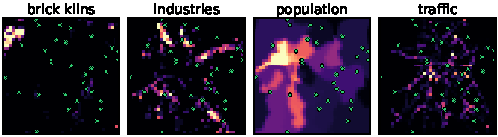
\includegraphics[width=\columnwidth]{figures/fig_platform.pdf}
\caption{Proxy maps of the four source groups on the \(40\times40\) grid (each
inventory map divided by its own 99th percentile, with colour clipped at \(1\)) and the 32
regulatory sensor cells (green).  Traffic is the mean of the four time-of-day road
maps.}
\label{fig:platform}
\end{figure}

\noindent\textbf{Transport operator.}
Emissions released at hour \(t-\ell\) reach the sensors at hour \(t\) after transport
by the wind between the two hours.  Let \(G_{t,t-\ell}\) map emissions on the source
grid at \(t-\ell\) to concentrations at the \(m\) sensors at \(t\) under an
open-boundary Gaussian-puff model driven by the gridded wind \(\omega\) (mass that
leaves the domain is removed), and let \(\mathbf s_k\) be the proxy map of group \(k\).
The PM\(_{2.5}\) that one unit of \(c_{kb}\) produces at the sensors at hour \(t\) is
\begin{equation}
\mathbf a_{t,kb}(\omega)=\sum_{\ell=0}^{\min(L,t-1)}\phi_b(t-\ell)\,G_{t,t-\ell}\,\mathbf s_k
\in\mathbb R^m.
\label{eq:transport_column}
\end{equation}
In \(G_{t,t-\ell}\), a unit release is advected along the interpolated wind and spread by
a Gaussian kernel, evaluated at the sensors, whose variances along and across the mean
wind grow as \(0.7^2\) and \(0.25^2\) square cells per hour of travel.  The model is
two-dimensional and treats PM\(_{2.5}\) as a passive primary tracer, without mixing
height, deposition or secondary formation (Appendix~\ref{app:transport_response}).  Stacking over
hours gives column \(\mathbf a_{kb}(\omega)\) of the operator \(A(\omega)\).  The lag is declared before fitting: \(L=12\) hours in every reported run except the lag
sweep of Experiment 7.

\noindent\textbf{Model, nuisance and projection.}
Let \(\mathbf y\in\mathbb R^N\) stack the observed hourly readings; rows with a missing
reading are removed from \(\mathbf y\), \(A(\omega)\) and \(Q\) alike.  The model is
\begin{equation}
\mathbf y = A(\omega)\,\mathbf c + Q\boldsymbol\gamma + \boldsymbol\epsilon,
\qquad \mathbf c\ge 0,
\label{eq:general_model}
\end{equation}
with \(\mathbf c\in\mathbb R_+^J\), free nuisance coefficients \(\boldsymbol\gamma\) and
noise \(\boldsymbol\epsilon\).  The nuisance basis \(Q\in\mathbb R^{N\times r}\) represents
regional background and smooth trends.  Except in the nuisance-basis variations of Experiments 3 and 11, it
has rank \(r=4\): a constant, a linear time trend and one daily sine--cosine pair,
declared before fitting and never built from the inventories or from fitted
signals.  With
\(P_Q^\perp=I-QQ^\dagger\), the projected problem is
\begin{equation}
\yt=\At\mathbf c+\widetilde{\boldsymbol\epsilon},\qquad
\yt=P_Q^\perp\mathbf y,\qquad
\At=P_Q^\perp A(\omega).
\label{eq:projected_model}
\end{equation}
The projected column \(\at_j=P_Q^\perp\mathbf a_j\), the \emph{fingerprint} of component
\(j\), is the part of its signal that the nuisance cannot reproduce, and because the
projection can absorb a signal, every diagnostic is computed from \(\At\).

\noindent\textbf{The attribution problem.}
Let \(E=\{1,\dots,J\}\) index the components and let \(\mathcal D\) be the declared
partition of \(E\) into source groups.  For \(g\subseteq E\), \(\At_g\) is the submatrix
of the columns in \(g\), and the \emph{signal} of \(g\) is \(\At_g\mathbf c_g\), its
contribution to the projected readings.  It is in \(\mu\mathrm g/\mathrm m^3\) and does
not change when a proxy map is rescaled; a sum of coefficients \(\sum_{j\in g}c_j\) has
neither property.  The task is to choose a partition \(\mathcal P\) of \(E\) whose blocks
are unions of blocks of \(\mathcal D\), using only \(\At\), \(\mathcal D\) and a declared
noise level, before the readings are fitted, and then to report for each block \(g\) its
fitted signal \(\At_g\widehat{\mathbf c}_g\), its share
\(\|\At_g\widehat{\mathbf c}_g\|_1/\sum_{h\in\mathcal P}\|\At_h\widehat{\mathbf c}_h\|_1\), and
the uncertainty of both.  The partition must meet two requirements.  (R1) \emph{Identifiability:} without
noise, the readings determine the signal of every block.  (R2) \emph{Reportability:} at
the declared noise level, the error of every block's fitted signal is bounded by a
stated multiple of the noise.  R1 excludes splits that no amount of data resolves, while R2 excludes splits that the
noise does not allow.  Section~\ref{sec:method} gives the procedure and
Section~\ref{sec:identifiability_theory} the conditions under which it meets both.

\section{Method: Identifiability-Aware Source Attribution}
\label{sec:method}
\label{sec:iasa_procedure}

IASA computes from \(\At\), before fitting, diagnostics and the partition to report,
then fits once (Algorithm~\ref{alg:iasa}, with thresholds in Table~\ref{tab:thresholds}).
Contributions are estimated by nonnegative least squares (NNLS),
\begin{equation}
\widehat{\mathbf c}=\arg\min_{\mathbf c\ge 0}\;\|\yt-\At\mathbf c\|_2^2,
\label{eq:nnls_estimator}
\end{equation}
solved by projected FISTA \citep{beck2009fast} (Appendix~\ref{app:pytorch_solver}), and
it is the same estimator in every experiment.

\noindent\textbf{Diagnostics.}
IASA reports the rank of \(\At\), its smallest singular value \(\sigma_J\) (zero if rank
deficient), \(\kappa=\sigma_1/\sigma_J\), the visibility \(\|\at_j\|_2\), the weak set of
columns with visibility at most \(\tau_v\) (\(\tau_v=0\) in every run), the absorption
\(\|P_Q\mathbf a_j\|_2/\|\mathbf a_j\|_2\), which is the fraction of a column that the
projection removes, and the coherence
\(\rho_{ij}=|\at_i^\top\at_j|/(\|\at_i\|_2\|\at_j\|_2)\).  The
central diagnostic is the \emph{separation} of a group \(g\subseteq E\),
\begin{equation}
s_g=\sin\theta_g ,
\label{eq:separation}
\end{equation}
where \(\theta_g\) is the smallest principal angle \citep{bjorck1973numerical} between
\(\operatorname{col}(\At_g)\) and \(\operatorname{col}(\At_{E\setminus g})\), with
\(s_g=1\) when either space is \(\{0\}\).  In words, \(s_g\) near \(0\) means that some signal of group \(g\) is nearly reproduced
by the other sources.  For an operator with two columns \(s=\sqrt{1-\rho^2}\), and for one
column \(1/s_j^2\) is the uncentered variance-inflation factor.  IASA raises an identifiability
\emph{flag} on a merge, a weak column, an absorption at least \(0.9\),
\(\sigma_J\le10^{-6}\) or a coherence at least \(0.99\).

\noindent\textbf{Grouping.}
The partition is chosen in two steps.  First, IASA computes the finest exactly
identifiable partition \(\mathcal P^\star\) of the columns
(Theorem~\ref{thm:groupings}(c)), and the blocks of \(\mathcal P^\star\vee\mathcal D\), the
finest partition coarser than both, are the \emph{atoms}.  Second, a partition into
unions of atoms is \emph{reportable} if every block has \(s_g\ge\tau_\theta\).  IASA
returns the reportable partition with the most blocks, breaks ties by the largest
smallest separation, and lists any remaining ties.  With \(q\le12\) atoms this search is
exact by dynamic programming in \(O(3^q)\) time, whereas with more atoms it merges greedily
(Appendix~\ref{app:identifiability_proofs}).  We use \(\tau_\theta=\sqrt{1-0.99^2}=0.141\),
so for an operator with two columns the rule merges exactly when their coherence
exceeds \(0.99\).  The recorded runs used either this rule or a pairwise rule that
merges declared blocks with a cross-source coherence above \(0.99\), and on every saved
operator and observed week the two rules give the same partition.

\begin{algorithm}[t]
\caption{Identifiability-Aware Source Attribution (IASA)}
\label{alg:iasa}
\footnotesize
\begin{algsteps}
  \item \textbf{Declare} \(Q\), components, \(\mathcal D\), \(\mathcal F_0\), \(L\),
  \(\sigma_e\), \(\delta\) and thresholds.
  \item \textbf{Operator:} build \(A(\omega)\) by~\eqref{eq:transport_column}.
  \item \textbf{Project:} drop rows with a missing reading and form \(\yt\),
  \(\At\)~\eqref{eq:projected_model}.
  \item \textbf{Diagnose:} singular values, rank, visibility, absorption, coherence,
  weak set.
  \item \textbf{Group:} \(\mathcal P^\star\), then atoms \(\mathcal P^\star\vee\mathcal D\),
  then the reportable partition at \(\tau_\theta\) with the most blocks.
  \item \textbf{Fit:} solve~\eqref{eq:nnls_estimator} and form group signals
  \(\At_g\widehat{\mathbf c}_g\) and shares.
  \item \textbf{Uncertainty:} error bound \(b_g\) of each block at \(\sigma_e\), bootstrap
  intervals of the shares, and a residual adequacy test if a calibrated noise model
  exists.
  \item \textbf{Report} group signals, shares, \(b_g\), intervals, coefficients of
  single-component blocks, diagnostics and flags.
\end{algsteps}
\end{algorithm}

\noindent\textbf{Uncertainty and adequacy.}
With a declared noise standard deviation \(\sigma_e\) per reading, IASA gives for each
reported block the bound
\(b_g=\sigma_e\bigl(\sqrt{\operatorname{rank}(\At)}+\sqrt{2\log(1/\delta)}\bigr)/s_g\) on
the error of its fitted signal, which holds with probability at least \(1-\delta\)
under the conditions of Theorem~\ref{thm:group_error}(c) (\(\delta=0.05\) here).  We
call a group's signal \emph{resolved} when \(b_g\) is below the norm of its fitted
signal.  It also gives percentile intervals
of the shares from a parametric bootstrap: since the NNLS estimate depends on the
readings only through \(P_{\At}\yt\), with \(P_{\At}\) the orthogonal projector onto
\(\operatorname{col}(\At)\), the bootstrap adds Gaussian noise of standard
deviation \(\sigma_e\) in \(\operatorname{col}(\At)\) to \(\At\widehat{\mathbf c}\) and
refits.  A residual adequacy test is run when a calibrated noise model exists,
and otherwise the residual is labelled uncalibrated (Appendix~\ref{app:reporting_details}).

\section{Theoretical Guarantees}
\label{sec:identifiability_theory}

This section gives the guarantees behind steps 2, 4, 5 and 7 of
Algorithm~\ref{alg:iasa}, and the proofs are in Appendix~\ref{app:identifiability_proofs}.
Steps 1--3 construct \(\At\) before any reading is fitted, and the analysis treats
\(\At\) as fixed, which requires the following.

\begin{assumption}[Declared model]
\label{ass:model}
\(\mathbf y\) follows~\eqref{eq:general_model} with \(\mathbf c\ge0\), where \(\mathbf y\)
is the readings minus a declared baseline field, and \(A(\omega)\), \(Q\), the components,
\(\mathcal F_0\) and the set of observed rows are fixed independently of
\(\boldsymbol\epsilon\).
\end{assumption}

In the observed runs the baseline is the transported field of a map interpolated from
the first hour of readings, and its error enters \(\boldsymbol\epsilon\).  The assumption
fails if \(Q\) or the components are chosen after looking at estimates, or if the
transport model is wrong (Section~\ref{subsec:operator_error}).  Step 7 also requires a
noise model.

\begin{assumption}[Noise]
\label{ass:noise}
\(\boldsymbol\epsilon\sim N(0,\sigma^2I_N)\) (or, where stated, \(N(0,\Sigma)\)), and the
declared level satisfies \(\sigma_e\ge\sigma\) (or \(\sigma_e^2\ge\|\Sigma\|_2\)).
\end{assumption}

On the observed data the difference of the two co-located monitors has lag-1
autocorrelation \(0.857\), so independence in time does not hold, and
\(\sigma_e\ge\sigma\) is not checked (Section~\ref{subsec:observed_results}).

\subsection{Individual Coefficients}

We begin with the individual source--basis coefficients, such as the four time-of-day
activities of traffic.

\begin{proposition}[Exact identifiability]
\label{prop:rank_identifiability}
In the noiseless projected model \(\yt=\At\mathbf c\), \(\At\mathbf c_1=\At\mathbf c_2\)
implies \(\mathbf c_1=\mathbf c_2\) for all \(\mathbf c_1,\mathbf c_2\in\mathbb R_+^J\)
if and only if \(\operatorname{rank}(\At)=J\).
\end{proposition}

\begin{proposition}[Noise robustness]
\label{prop:noise_robust}
Assume \(\operatorname{rank}(\At)=J\) and let \(\sigma_J(\At)\) be the smallest
singular value.  If \(\widehat{\mathbf c}\) is the least-squares estimate, or the
nonnegative least-squares (NNLS) estimate and \(\mathbf c\ge0\), then
\begin{equation}
\|\widehat{\mathbf c}-\mathbf c\|_2\le\|P_{\At}\widetilde{\boldsymbol\epsilon}\|_2/\sigma_J(\At)
\le\|\widetilde{\boldsymbol\epsilon}\|_2/\sigma_J(\At).
\label{eq:nnls_noise_bound}
\end{equation}
\end{proposition}

\begin{remark}[Implication: coefficients]
Both propositions require only Assumption~\ref{ass:model}.  In every observed week
\(\operatorname{rank}(\At)=7=J\).  With noise, \(1/\sigma_J\) is the largest factor by
which noise enters the coefficients, so an identifiable problem can still have large
coefficient errors (Experiment 1).  IASA reports \(\sigma_J\) in step 4 and reports coefficients only for
single-component blocks.
\end{remark}

\subsection{Identifiable Groupings}

When the coefficients are not determined, the reported quantity is the signal of a
group of sources.  The following definition states when such signals are determined,
which is requirement R1.

\begin{definition}[Identifiable grouping]
\label{def:identifiable_grouping}
A partition \(\mathcal P\) of \(E\) is \emph{identifiable} if
\(\At\mathbf c_1=\At\mathbf c_2\) with \(\mathbf c_1,\mathbf c_2\in\mathbb R_+^J\)
implies \(\At_g\mathbf c_{1,g}=\At_g\mathbf c_{2,g}\) for every block
\(g\in\mathcal P\).
\end{definition}

\begin{theorem}[Identifiable groupings]
\label{thm:groupings}
\leavevmode
\begin{enumerate}[label=(\alph*),leftmargin=*,itemsep=0pt,topsep=2pt]
  \item \(\mathcal P\) is identifiable if and only if
  \(\operatorname{col}(\At)=\bigoplus_{g\in\mathcal P}\operatorname{col}(\At_g)\),
  equivalently \(\operatorname{rank}(\At)=\sum_{g\in\mathcal P}\operatorname{rank}(\At_g)\).
  \item There is a unique finest identifiable partition \(\mathcal P^\star\), and
  \(\mathcal P\) is identifiable if and only if every block of \(\mathcal P\) is a
  union of blocks of \(\mathcal P^\star\).
  \item Let \(B\subseteq E\) index a basis of \(\operatorname{col}(\At)\) chosen from
  the columns, and join each \(e\notin B\) to every \(b\in B\) whose coefficient is
  nonzero when \(\at_e\) is written in that basis.  The blocks of \(\mathcal P^\star\)
  are the connected components of this graph, for any choice of \(B\), and they are the
  connected components of the column matroid of \(\At\).
  \item For a declared partition \(\mathcal D\), the finest identifiable partition
  whose blocks are unions of blocks of \(\mathcal D\) is the finest common coarsening
  \(\mathcal P^\star\vee\mathcal D\).
\end{enumerate}
\end{theorem}

\begin{remark}[Implication: exact resolution]
The theorem requires only Assumption~\ref{ass:model}.  A partition meets R1 exactly when no
group's span meets the span of the other groups except at \(0\) (a), and there is one
finest such partition (b), computed before fitting in \(O(NJ^2)\) arithmetic (c).  A source
shares its block of \(\mathcal P^\star\vee\mathcal D\) with another source exactly when a
nonzero combination of its fingerprints equals a combination of the other
fingerprints.  In every observed week \(\mathcal P^\star\) is the seven single columns,
so the atoms are the four groups.  Step 5 forms its atoms by (c) and (d), so every
partition IASA can return meets R1.  For sums of coefficients, which are in different
proxy units, the minimal groupings can be non-unique and deciding whether one with at
least two blocks exists is NP-complete (Proposition~\ref{prop:sum_identifiable},
Appendix~\ref{app:identifiability_proofs}), so IASA reports signals instead.
\end{remark}

\subsection{Group-Signal Error}

Requirement R2 concerns the effect of noise, which identifiability does not control.
The error of a group's fitted signal is governed by its separation \(s_g\)
of~\eqref{eq:separation}, not by \(\sigma_J\).

\begin{theorem}[Group-signal error]
\label{thm:group_error}
Let \(\mathcal P\) be identifiable and let \(\widehat{\mathbf c}\) be any
least-squares solution, or any NNLS solution with \(\mathbf c\ge0\).
\begin{enumerate}[label=(\alph*),leftmargin=*,itemsep=0pt,topsep=2pt]
  \item The group signals \(\At_g\widehat{\mathbf c}_g\) do not depend on which
  solution is chosen, and for every \(g\in\mathcal P\),
  \begin{equation}
  \|\At_g(\widehat{\mathbf c}_g-\mathbf c_g)\|_2
  \le
  \frac{\|P_{\At}\widetilde{\boldsymbol\epsilon}\|_2}{s_g}.
  \label{eq:group_bound}
  \end{equation}
  \item If \(\boldsymbol\epsilon\sim N(0,\sigma^2I_N)\), for a least-squares solution and
  \(r_g=\operatorname{rank}(\At_g)\),
  \(\mathbb E\|\At_g(\widehat{\mathbf c}_g-\mathbf c_g)\|_2^2\le\sigma^2r_g/s_g^2\), with
  equality when \(r_g=1\).
  \item If \(\boldsymbol\epsilon\sim N(0,\sigma^2I_N)\), with probability at least
  \(1-\delta\), simultaneously for every identifiable partition and every block \(g\),
  \begin{equation}
  \|\At_g(\widehat{\mathbf c}_g-\mathbf c_g)\|_2
  \le
  \frac{\sigma\bigl(\sqrt{\operatorname{rank}(\At)}+\sqrt{2\log(1/\delta)}\bigr)}{s_g},
  \label{eq:group_bound_gauss}
  \end{equation}
  and if \(\boldsymbol\epsilon\sim N(0,\Sigma)\), the same holds with \(\sigma^2\)
  replaced by \(\|\Sigma\|_2\).
\end{enumerate}
\end{theorem}

\begin{remark}[Implication: the error bound IASA reports]
Part (a) holds for every noise vector under Assumption~\ref{ass:model}, whereas (b) and
(c) also need the Gaussian noise of Assumption~\ref{ass:noise}.  IASA, which uses NNLS, relies on
(a) and (c).  The columns inside a group, such as the four time-of-day columns of
traffic, can be nearly dependent, which makes the bound of
Proposition~\ref{prop:noise_robust} large while the group's signal error stays at most
\(\|P_{\At}\widetilde{\boldsymbol\epsilon}\|_2/s_g\).  With \(\sigma\) replaced by the
declared \(\sigma_e\), the right side of~\eqref{eq:group_bound_gauss} is the bound
\(b_g\) of step 7, which holds when \(\sigma_e\ge\sigma\) and the operator is exact.  Requiring \(b_g\le\eta\) for a tolerance \(\eta\) gives
the threshold \(\tau_\theta=\sigma_e(\sqrt{\operatorname{rank}(\At)}+\sqrt{2\log(1/\delta)})/\eta\)
of step 5, and \(0.141\) corresponds to \(\eta=7.1\,\sigma_e(\sqrt{\operatorname{rank}(\At)}+\sqrt{2\log(1/\delta)})\).
\end{remark}

\begin{definition}[Reportable partition]
\label{def:reportable}
A partition into unions of atoms is \emph{reportable at threshold
\(\tau_\theta\in(0,1]\)} if every block has \(s_g\ge\tau_\theta\).
\end{definition}

Reportable partitions are not closed under coarsening, and the minimal ones (with no
strictly finer reportable partition) need not be unique
(Proposition~\ref{prop:reportable_structure}), so with up to 12 atoms IASA checks every
union of atoms and lists ties.  The one-block partition is always reportable.

\subsection{Errors in the Operator}
\label{subsec:operator_error}

The operator is built from an estimated wind field and assumed dispersion parameters.
The next result bounds how far an error \(\Delta\) in \(\At\) moves the separations.

\begin{proposition}[Stability under operator error]
\label{prop:grouping_stability}
Let \(\At'=\At+\Delta\).  For \(S\subseteq E\) with \(\At_S\) of full column rank and
\(\|\Delta_S\|_2\le\sigma_{\min}(\At_S)/2\), let
\(\beta_S=\arcsin\bigl(\|\Delta_S\|_2/(\sigma_{\min}(\At_S)-\|\Delta_S\|_2)\bigr)\).
If this holds for \(S=g\) and \(S=E\setminus g\), with \(g\) nonempty and proper, then
\(|\theta_g(\At')-\theta_g(\At)|\le\beta_g+\beta_{E\setminus g}\).  If \(\At\) has full
column rank, \(\|\Delta\|_2\le\sigma_J(\At)/2\), and
\(|\theta_g(\At)-\arcsin\tau_\theta|>\beta_g+\beta_{E\setminus g}\) for every nonempty
proper union \(g\) of atoms, the reportable partitions of \(\At'\) and \(\At\) coincide,
and so do the minimal reportable partitions.
\end{proposition}

\begin{remark}[Implication: wind and dispersion error]
The proposition uses no noise assumption.  Under a wind or dispersion error \(\Delta\) that meets
the conditions, the set of reportable partitions is unchanged, and so is the reported
partition when one reportable partition has the most blocks.  In every observed week
each union of atoms has a separation angle of at least \(45.4^\circ\), against
\(\arcsin\tau_\theta=8.1^\circ\), but whether the true \(\Delta\) meets the conditions is not
known.
The fitted signals do change: for least squares, an operator error acts as additional
noise of size at most \(\|\Delta\|_2\|\mathbf c\|_2\)
(Proposition~\ref{prop:operator_perturbation}, Appendix~\ref{app:operator_error_details}),
which Experiment 5 measures.
\end{remark}

\section{Experiments}
\label{sec:application}

We evaluate IASA in controlled experiments with known contributions
(Section~\ref{subsec:pollution_controlled}) and on four observed weeks without ground
truth (Section~\ref{subsec:observed_results}).

\subsection{Controlled Experiments}
\label{subsec:pollution_controlled}

The controlled experiments generate PM\(_{2.5}\) readings from known nonnegative
contributions with the puff model of Section~\ref{sec:problem_setup} on the
\(40\times40\) grid, so that the error of every reported quantity can be measured.  Each
run covers 72 hours, mostly with two source groups, and varies one factor at a time:
wind, sensor layout, nuisance basis, noise, operator error, lag, temporal basis or
inventory.  Unless the factor is varied, the sensors are the 32 regulatory locations,
with three downwind sensors in Experiment 10 and six random ones in the steady-wind
case of Experiment 11.  The sources are compact synthetic emitters except in
Experiments 2, 6 and 8, which use the New Delhi maps, and the winds are synthetic
except where real wind is stated
(Appendices~\ref{app:pollution_experiments}--\ref{app:additional_experiments}).  Coefficient error is
\(\|\widehat{\mathbf c}-\mathbf c\|_2/\|\mathbf c\|_2\), the group-signal error of a
reported block \(G\) is \(\|\At_G(\widehat{\mathbf c}_G-\mathbf c_G)\|_2/\|\At_G\mathbf c_G\|_2\),
and noise is Gaussian with standard deviation stated as a fraction of the largest
absolute noiseless source signal of that run.

\begin{figure*}[t]
\centering
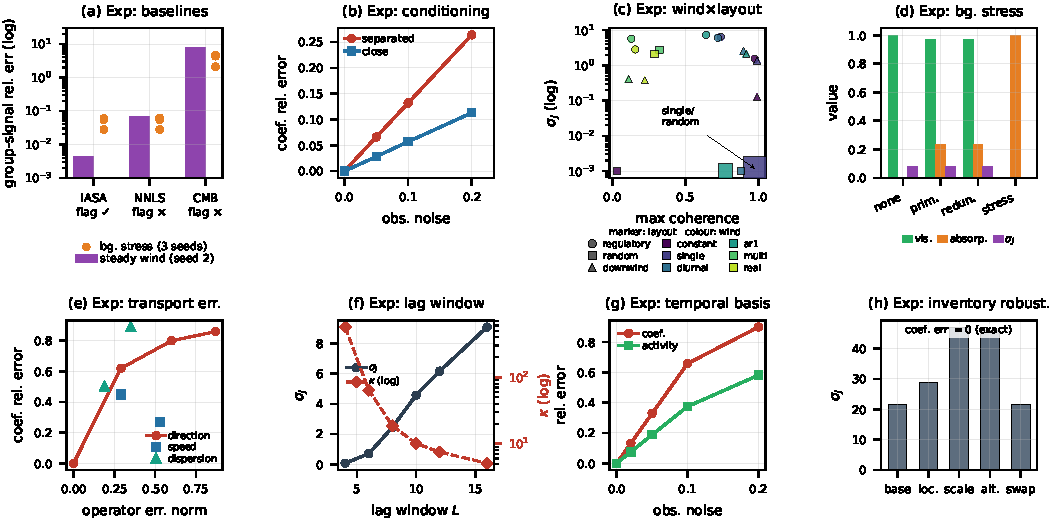
\includegraphics[width=\textwidth]{figures/fig_controlled.pdf}
\caption{Controlled experiments on the New Delhi platform.  \textbf{(a)}~Largest
relative group-signal error of IASA and two baselines that raise no identifiability
flag (plain NNLS on the projected system, a mass balance on the unprojected
response): background stress over three seeds (points) and the steady-wind case in the
seed where the plumes reach the sensors (bars).  \textbf{(b)}~Coefficient error against
noise for two sources \(4\) cells apart (\(\sigma_J=9.6\), \(\kappa=2.3\)) and \(20\)
cells apart (\(\sigma_J=3.3\), \(\kappa=8.9\)).  \textbf{(c)}~\(\sigma_J\) against maximum
coherence across wind providers (colour, with ar1 denoting AR(1) wind) and sensor
layouts (marker), where marker size increases with coefficient error and \(\sigma_J\)
below \(10^{-3}\) is drawn at \(10^{-3}\).  \textbf{(d)}~Nuisance bases none, primary
(rank 4), redundant (same span) and stress (source-like column): the stress basis drives
absorption to \(1\) and \(\sigma_J\) and the visibility ratio
\(\|\at_j\|_2/\|\mathbf a_j\|_2\) to \(0\).
\textbf{(e)}~Coefficient error against operator-error norm along the wind-direction,
wind-speed and dispersion axes.  \textbf{(f)}~\(\sigma_J\) and \(\kappa\) against the lag
window.  \textbf{(g)}~Activity error and coefficient error against noise.
\textbf{(h)}~\(\sigma_J\) across inventory versions.}
\label{fig:controlled}
\end{figure*}

\noindent\textbf{Baselines on two controlled degeneracies.}
IASA is compared over three seeds with plain NNLS on the projected system (the same
estimator without grouping and diagnostics), a transport-based mass balance (CMB: NNLS
on the unprojected response, with transport columns in place of chemical profiles) and
a nonnegative matrix factorization of the sensor-by-hour readings (PMF/NMF)
(Figure~\ref{fig:controlled}(a), Table~\ref{tab:results_baselines}).  Every method is
scored on IASA's reported blocks, errors range over those blocks, and share error is
the \(L_2\) distance between share vectors.  \emph{Source-like background} (32 regulatory
sensors, two sources with two columns each): a declared nuisance column is
proportional to one basis column of source A, whose norm falls from \(0.081\) to
\(10^{-16}\) under projection.  IASA flags it (absorption \(1\)), the two sources
have separation above \(0.9999\), and IASA's group-signal errors are
\(0.4\)--\(6.0\%\), with share errors \(0.003\)--\(0.007\).  Plain
NNLS gives group-signal errors within \(0.003\) of IASA's and raises no flag.  CMB,
without nuisance removal, has group-signal errors of \(36\)--\(463\%\) and share errors
\(0.12\)--\(0.19\).  \emph{Steady wind}
(one wind direction, six random sensors): in two seeds neither plume reaches the
sensors (column norms below \(10^{-10}\), against \(0.062\) and \(0.067\) in the third), and
IASA flags \(\sigma_J\approx0\).  In the third seed the two columns have coherence
\(0.99966\) and separation \(0.026<\tau_\theta\), so no reportable partition has two
blocks.  IASA therefore merges them, and the merged signal has error \(0.44\%\), against
\(784\%\) for CMB.
Reported separately, as plain NNLS reports them, the two sources' signals have errors of
\(3.8\%\) and \(6.9\%\).  PMF/NMF has share errors on the unprojected response of
\(1.15\)--\(1.19\) (background stress) and \(0.30\) (steady wind), and no baseline raises
a flag in either scenario.

\begin{table}[t]
\centering
\footnotesize
\setlength{\tabcolsep}{3pt}
\caption{Experiment 11: largest relative group-signal error of the reported blocks
(background stress in seeds \(0\), \(1\) and \(2\), and steady wind in seed \(2\), the only
seed with signal at the sensors).  Share errors: Table~\ref{tab:results_baselines_full}.}
\label{tab:results_baselines}
\vspace{3pt}
\begin{tabular}{llcc}
\toprule
method & flag & background stress & steady wind \\
\midrule
IASA & yes & \(0.054,\,0.028,\,0.060\) & \(0.004\) (merged) \\
plain NNLS & no & \(0.054,\,0.028,\,0.062\) & \(0.004\) \\
CMB & no & \(4.63,\,2.10,\,4.32\) & \(7.84\) \\
\bottomrule
\end{tabular}
\end{table}

\noindent\textbf{Conditioning and noise (Experiment 1).}
For two full-rank geometries, coefficient error is zero without noise and grows
linearly with it (one noise draw, scaled): \(0.066\), \(0.132\), \(0.264\) at noise
\(0.05\), \(0.10\), \(0.20\) for \(\sigma_J=3.27\), against \(0.028\), \(0.057\), \(0.113\)
for \(\sigma_J=9.60\) (Figure~\ref{fig:controlled}(b), Table~\ref{tab:results_h1}),
consistent with Proposition~\ref{prop:noise_robust}.

\noindent\textbf{Sensor layout and wind (Experiment 4).}
With the 32 regulatory locations, \(\sigma_J\ge1.53\) under all six winds, and the
maximum coherence falls from \(0.975\) under a constant wind to \(0.129\) and \(0.156\)
under multi-directional and real New Delhi wind (Figure~\ref{fig:controlled}(c),
Table~\ref{tab:results_h4}).  With eight randomly placed sensors and four of the six
winds, source B's operator column has norm \(5.2\times10^{-7}\) to \(1.7\times10^{-4}\),
against \(7.6\)--\(18.6\) with the regulatory layout, so \(\sigma_J\approx0\) and the
largest coefficient error of the sweep (\(0.573\)) is that source's poorly determined
coefficient (\(\sigma_J\approx10^{-6}\)).  The layouts also differ in sensor count.

\noindent\textbf{Nuisance absorption and missing sources (Experiments 3 and 8).}
A source-like nuisance basis drives the absorption of one column to \(1\) and
\(\sigma_J\) to \(0\) while the fitted residual is unchanged (Figure~\ref{fig:controlled}(d),
Table~\ref{tab:results_h3}), and the coefficient error falls (\(0.78\) with the
source-like basis against \(2.61\) with the rank-4 basis) because the signal has been
absorbed, so the error alone would not reveal the problem.
The adequacy test (\(\alpha=0.05\), \(1{,}000\) replicates) rejects at rate \(0.05\) under
a correct model and \(1.00\) when an omitted source has \(91\%\) of its signal outside the
span of \(A(\omega)\) and \(Q\), whereas an omitted source equal to a nonnegative
combination of the fitted columns plus nuisance columns is absorbed and rejected at rate
\(0.05\)
(Table~\ref{tab:results_missing}).  A non-rejection therefore does not show that the inventory is complete.

\noindent\textbf{Transport error (Experiment 5).}
This experiment measures the operator error of
Proposition~\ref{prop:operator_perturbation}.  Fitting with a perturbed operator
(Figure~\ref{fig:controlled}(e), Table~\ref{tab:results_h5a}), the coefficient error reaches \(0.62\) at a \(5^\circ\) error in wind
direction, \(0.86\) at \(20^\circ\) and \(0.89\) at twice the dispersion, while along the
speed axis it is not monotonic (\(0.45\) at \(1.25\times\), \(0.27\) at
\(1.5\times\)).  A structural mismatch (advection--diffusion data, puff operator) is rejected in
\(100\%\) of trials.

\noindent\textbf{Lag, temporal basis and inventory (Experiments 7, 9 and 6).}
From \(L=4\) to \(16\) hours \(\sigma_J\) rises from \(0.08\) to \(9.07\), but the operator
still changes by \(6\)--\(14\%\) between adjacent lags (Figure~\ref{fig:controlled}(f)).
Activity trajectories have lower error than coefficients (\(0.58\) against \(0.90\) at
\(20\%\) noise, panel (g)), and \(\sigma_J\) moves from \(21.6\) to \(47.0\) under a
rescaled inventory map while recovery stays exact (panel (h)).

\subsection{Observed New Delhi Weeks}
\label{subsec:observed_results}

\noindent\textbf{Data.}
We fit the first four weeks of the record, 1--28 May 2018, separately.  Each uses the
\(79\)--\(85\%\) of sensor-hours with a valid reading (\(N=4{,}236\)--\(4{,}561\)) and
\(J=7\) columns after \(\mathcal F_0\): one temporal component each for brick kilns,
industries and population, and four time-of-day components for traffic.  The declared
partition \(\mathcal D\) has one block per source group.  A transported
initial-condition field is subtracted (Appendix~\ref{app:platform_details}), and there
is no ground truth.

\noindent\textbf{Noise level.}
The two co-located monitors at Pusa differ with standard deviation
\(43.4\,\mu\mathrm g/\mathrm m^3\) over \(17{,}949\) shared hours (none in May 2018).  If
their errors are independent with equal variance, each has
\(\sigma_e=43.4/\sqrt2=30.7\,\mu\mathrm g/\mathrm m^3\).  The difference has lag-1
autocorrelation \(0.857\) (Appendix~\ref{app:observed_full}).  \(\sigma_e\) describes
instrument error at one site, and operator error adds to it.

\noindent\textbf{Identifiable resolution.}
Every week has numerical rank \(7\) of \(7\), so \(\mathcal P^\star\) is the seven
single columns and \(\mathcal P^\star\vee\mathcal D\) is the four source groups.  No
fingerprint is zero, \(\sigma_J\) is \(3.71\)--\(10.15\), and the largest pairwise
coherence is \(0.316\)--\(0.496\), so no merge, weak-column, \(\sigma_J\) or coherence flag
is raised (absorption was not recorded).  Every group has separation
\(0.72\)--\(0.96\ge\tau_\theta\), so IASA reports the four groups in every week
(Figure~\ref{fig:observed}(a)).  At \(\sigma_e=30.68\), \(\tau_\theta\) corresponds to
\(\eta\approx1{,}100\,\mu\mathrm g/\mathrm m^3\), above every fitted group norm, so the
noise statement comes from \(b_g\), not from the grouping.

\begin{figure}[t]
\centering
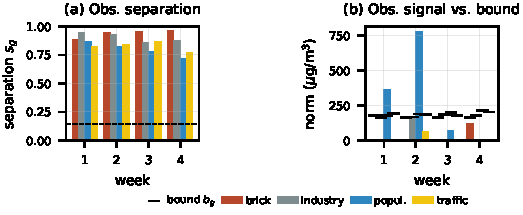
\includegraphics[width=\columnwidth]{figures/fig_observed.pdf}
\caption{Observed New Delhi, weeks 1--4.  \textbf{(a)}~Separation \(s_g\) of each source
group, with the dashed line at \(\tau_\theta=0.141\).  \textbf{(b)}~Norm of each fitted group signal
over the week's readings (bars) and its error bound \(b_g\) of
Theorem~\ref{thm:group_error}(c) at \(\sigma_e=30.68\), \(\delta=0.05\) (ticks).}
\label{fig:observed}
\end{figure}

\noindent\textbf{Group signals against the noise level.}
Theorem~\ref{thm:group_error}(c) with \(\sigma_e=30.68\), \(\operatorname{rank}(\At)=7\)
and \(\delta=0.05\) bounds the error of each group's fitted signal by
\(b_g=156.2/s_g\), which is \(162\)--\(217\,\mu\mathrm g/\mathrm m^3\) for the four groups
(Figure~\ref{fig:observed}(b)).  For the largest group, \(b_g\) is \(0.49\) and \(0.24\)
times its fitted norm in weeks 1 and 2 (population, with norms \(365\) and \(776\)) and
\(2.96\) and \(1.33\) times it in weeks 3 and 4 (population with norm \(67.5\) and brick
kilns with norm \(121.5\)).  At this noise level the bound therefore establishes that the largest group's signal is
resolved in weeks 1 and 2, and does not establish it in weeks 3 and 4.  The bootstrap gives the same split
(Table~\ref{tab:observed_shares}): the 95\% interval of the largest share has width
\(0.25\) and \(0.14\) in weeks 1 and 2, and \(0.94\) and \(0.67\) in weeks 3 and 4.  For AR(1) errors with coefficient \(0.857\), independent across sensors,
\(\|\Sigma\|_2\le(1+0.857)/(1-0.857)\,\sigma_e^2=13.0\,\sigma_e^2\), a level of \(110.7\),
at which the bound exceeds the largest group's norm in every week except week 2.

\noindent\textbf{What the fit explains.}
The projected residual has root mean square \(46\)--\(91\,\mu\mathrm g/\mathrm m^3\) per
reading, against \(1.05\)--\(13.24\) for the total fitted signal (\(2.3\)--\(14.5\%\) of the
residual in each week).  The adequacy test reports no verdict because no calibrated noise model exists.  The bounds above hold under
Assumptions~\ref{ass:model} and~\ref{ass:noise}, and a residual root mean square
\(1.5\)--\(3.0\) times \(\sigma_e\) means that the declared model, the noise level, or both
do not describe these weeks fully.  The shares are fractions of the fitted projected
concentration signal, so they are not emission shares, and because the nuisance terms
are removed first they are not shares of PM\(_{2.5}\) mass.

\section{Conclusion}
\label{sec:discussion_conclusion}

We attributed PM\(_{2.5}\) from a regulatory network to declared source groups at the
resolution that the projected transport operator supports.  The finest exactly
identifiable grouping is unique and is computed before fitting, and the error of each
reported group's signal is bounded by the noise divided by its separation.  In
controlled experiments the procedure flagged the two situations in which the mass
balance without background removal had group-signal errors of \(36\)--\(784\%\).  On the
observed New Delhi weeks, the four source groups are separable in
every week, but at the instrument noise level the error bound of the largest group's
signal is below its fitted norm in two of four weeks and above it in the other two.  With
historical wind, the diagnostics can assess a sensor layout before deployment.

\noindent\textbf{Limitations.}
All results are conditional on the declared wind, transport model, inventories and
nuisance basis.  The shares are fractions of the fitted projected
concentration signal, not shares of emissions or of PM\(_{2.5}\) mass, and
on the observed weeks the fitted signal is \(2.3\)--\(14.5\%\) of the residual in root mean
square.  An omitted source can be absorbed by the fit without detection.  The noise level comes
from one pair of co-located monitors over a record that excludes the study weeks, and
the bounds and the bootstrap assume Gaussian noise and an exact operator.  The transport
model is two-dimensional, without mixing height, deposition or secondary formation, and
dust, biomass burning and secondary aerosol are not declared.  Sensitivity of the
observed results to the lag, nuisance basis and dispersion is not reported, the gridded
wind is not validated against dense measurements, and the controlled experiments
do not compare \(b_g\) or bootstrap coverage with known errors.  The observed study
covers four weeks of May 2018 without ground truth.  The
network's gas measurements are not used and could serve as additional tracers.


\subsection*{AI use statement}

% AUTHORS: this draft records the AI use in the AISTATS revision only.  Confirm every
% sentence, and add any AI use in earlier versions of the work, before submission.
In this work, we used generative AI tools (Claude, Anthropic) for writing code (the
grouping module and its tests), for restructuring and
editing the manuscript, for literature search and checking bibliographic entries, and
for drafting proofs and checking them numerically on random instances.  We have not
used generative AI tools to generate, modify or label data.  All AI-assisted code was
run and tested, every reported number was regenerated from the released code and the
committed results, and the proofs were checked by the authors.  We take responsibility
for the final content of this work, including text, claims, or artifacts produced with
the aid of generative AI.


% Acknowledgements are included only in the camera-ready version (anonymous review).

\bibliography{refs}

\section*{Checklist}

% AUTHORS: confirm each answer before submission; the anonymized code archive is the
% one item that still has to be produced.
\begin{enumerate}

  \item For all models and algorithms presented, check if you include:
  \begin{enumerate}
    \item A clear description of the mathematical setting, assumptions, algorithm,
    and/or model. [Yes; Sections~\ref{sec:problem_setup}
    and~\ref{sec:identifiability_theory}, Algorithm~\ref{alg:iasa},
    Appendix~\ref{app:reporting_details}.]
    \item An analysis of the properties and complexity (time, space, sample size) of
    any algorithm. [Yes; Theorem~\ref{thm:groupings} and the text after it
    (\(O(NJ^2)\) for the exact components).]
    \item (Optional) Anonymized source code, with specification of all dependencies,
    including external libraries. [Yes; supplementary archive with
    \texttt{model/iasa}, \texttt{experiments/} and the dependency list (Python 3.12,
    PyTorch, NumPy, SciPy, pandas, scikit-learn, einops, Matplotlib).]
  \end{enumerate}

  \item For any theoretical claim, check if you include:
  \begin{enumerate}
    \item Statements of the full set of assumptions of all theoretical results. [Yes;
    each statement in Section~\ref{sec:identifiability_theory} and
    Appendix~\ref{app:identifiability_proofs} lists its assumptions.]
    \item Complete proofs of all theoretical results. [Yes;
    Appendix~\ref{app:identifiability_proofs}.]
    \item Clear explanations of any assumptions. [Yes.]
  \end{enumerate}

  \item For all figures and tables that present empirical results, check if you
  include:
  \begin{enumerate}
    \item The code, data, and instructions needed to reproduce the main experimental
    results (either in the supplemental material or as a URL). [Yes; supplementary
    code and configurations; the PM\(_{2.5}\) and wind records are public CPCB data
    \citep{cpcb,cpcb_portal}.]
    \item All the training details (e.g., data splits, hyperparameters, how they were
    chosen). [Yes; thresholds in Table~\ref{tab:thresholds}, solver settings in
    Appendix~\ref{app:pytorch_solver}.]
    \item A clear definition of the specific measure or statistics and error bars
    (e.g., with respect to the random seed after running experiments multiple times).
    [Yes; metrics are defined where reported; Experiment 11 is over three seeds, and
    the observed shares carry 95\% parametric-bootstrap intervals.]
    \item A description of the computing infrastructure used. (e.g., type of GPUs,
    internal cluster, or cloud provider). [Yes; Appendix~\ref{app:reproducibility}: Experiment 11 and the observed
    re-analysis ran on one laptop CPU (Apple M5); the other controlled
    experiments and the observed fits ran on an NVIDIA GPU with CUDA 11.8, and the
    controlled experiments reproduce on CPU.]
  \end{enumerate}

  \item If you are using existing assets (e.g., code, data, models) or
  curating/releasing new assets, check if you include:
  \begin{enumerate}
    \item Citations of the creator If your work uses existing assets. [Yes; CPCB data,
    emission inventories and the population grid are cited.]
    \item The license information of the assets, if applicable. [Yes;
    Appendix~\ref{app:reproducibility}.]
    \item New assets either in the supplemental material or as a URL, if applicable.
    [Yes; code in the supplementary archive.]
    \item Information about consent from data providers/curators. [Not Applicable;
    public government records.]
    \item Discussion of sensible content if applicable, e.g., personally identifiable
    information or offensive content. [Not Applicable.]
  \end{enumerate}

  \item If you used crowdsourcing or conducted research with human subjects, check if
  you include:
  \begin{enumerate}
    \item The full text of instructions given to participants and screenshots. [Not
    Applicable.]
    \item Descriptions of potential participant risks, with links to Institutional
    Review Board (IRB) approvals if applicable. [Not Applicable.]
    \item The estimated hourly wage paid to participants and the total amount spent on
    participant compensation. [Not Applicable.]
  \end{enumerate}

\end{enumerate}


\clearpage
\appendix
\thispagestyle{empty}
\onecolumn
\aistatstitle{Identifiability-Aware Source Attribution of Air Pollution:\\
Supplementary Materials}

\section{Proofs}
\label{app:identifiability_proofs}

In this appendix \(A\) denotes the projected operator \(\widetilde A\) of
Equation~\ref{eq:projected_model}, \(\mathbf a_j\) its columns,
\(V_g=\operatorname{col}(A_g)\), \(W_g=\operatorname{col}(A_{E\setminus g})\) and
\(U=\operatorname{col}(A)\).  The unit tests in the code release
(\texttt{tests/test\_iasa\_grouping.py}) check numerically the exact components against
brute force (Theorem~\ref{thm:groupings}(b)--(d)), the two-column separation
\(\sqrt{1-\rho^2}\), Theorem~\ref{thm:group_error}(a), the examples of
Proposition~\ref{prop:reportable_structure}, and the exhaustive and greedy partition
searches.

\subsection{Individual Contributions}

\noindent\textbf{Proof of Proposition~\ref{prop:rank_identifiability}.}
If \(\operatorname{rank}(A)=J\), the rank--nullity theorem gives
\(\ker(A)=\{\mathbf 0\}\), so \(A\mathbf c_1=A\mathbf c_2\) implies
\(\mathbf c_1=\mathbf c_2\).  Conversely, if \(\operatorname{rank}(A)<J\) there is a
nonzero \(\mathbf d\in\ker(A)\).  Choose \(\beta>\|\mathbf d\|_\infty\) and set
\(\mathbf c=\beta\mathbf 1\).  Then \(\mathbf c\) and \(\mathbf c+\mathbf d\) are
distinct, both lie in \(\mathbb R_+^J\) because
\(\beta+d_j\ge\beta-\|\mathbf d\|_\infty>0\), and
\(A(\mathbf c+\mathbf d)=A\mathbf c\).  \(\square\)

The same interior-point construction is used below whenever a kernel vector must be
turned into two nonnegative vectors with equal projected observations.

\noindent\textbf{Proof of Proposition~\ref{prop:noise_robust}.}
For least squares with full column rank,
\(\widehat{\mathbf c}-\mathbf c=A^\dagger\widetilde{\boldsymbol\epsilon}
=A^\dagger P_A\widetilde{\boldsymbol\epsilon}\), and
\(\|A^\dagger\|_2=1/\sigma_J(A)\).  For NNLS, let
\(C=\{A\mathbf z:\mathbf z\ge0\}\), a closed convex cone contained in \(U\).  For
\(\mathbf x\in U\),
\(\|\yt-\mathbf x\|_2^2=\|P_A\yt-\mathbf x\|_2^2+\|(I-P_A)\yt\|_2^2\), so the
fitted signal is \(A\widehat{\mathbf c}=\Pi_C(\yt)=\Pi_C(P_A\yt)\), where \(\Pi_C\) is
the Euclidean projection onto \(C\).  Since \(\mathbf c\ge0\), \(A\mathbf c\in C\)
and \(\Pi_C(A\mathbf c)=A\mathbf c\).  Projection onto a closed convex set is
nonexpansive, so
\[
\|A(\widehat{\mathbf c}-\mathbf c)\|_2
=\|\Pi_C(P_A\yt)-\Pi_C(A\mathbf c)\|_2
\le\|P_A\yt-A\mathbf c\|_2
=\|P_A\widetilde{\boldsymbol\epsilon}\|_2 .
\]
Full column rank gives \(\|A\Delta\|_2\ge\sigma_J(A)\|\Delta\|_2\) for
\(\Delta=\widehat{\mathbf c}-\mathbf c\), which proves the first inequality
in~\eqref{eq:nnls_noise_bound}; the second holds because \(P_A\) is an orthogonal
projector.  \(\square\)

\noindent\textbf{Ray distance (Equation~\ref{eq:ray_distance_coherence_relation}).}
For nonzero \(\mathbf a_i,\mathbf a_j\), the function
\(\alpha\mapsto\|\mathbf a_i-\alpha\mathbf a_j\|_2^2/\|\mathbf a_i\|_2^2\) is
strictly convex with minimizer
\(\alpha^\star=\mathbf a_i^\top\mathbf a_j/\|\mathbf a_j\|_2^2\) and minimum
\(1-\rho_{ij}^2\).  The minimum is also \(\sin^2\) of the angle between
\(\mathbf a_i\) and \(\operatorname{span}(\mathbf a_j)\), so for \(J=2\) the ray
distance equals the sine of the angle between the two columns.  \(\square\)

\noindent\textbf{Proof of Proposition~\ref{prop:operator_perturbation}.}
Let \(\widehat A\) have full column rank and \(\|\widehat A-A^\star\|_2\le\delta_H\).
The data obey
\(\yt=A^\star\mathbf c+\widetilde{\boldsymbol\epsilon}
=\widehat A\mathbf c+[\widetilde{\boldsymbol\epsilon}+(A^\star-\widehat A)\mathbf c]\),
and \(\widehat A^\dagger\widehat A=I_J\), so
\(\widehat{\mathbf c}-\mathbf c=\widehat A^\dagger[\widetilde{\boldsymbol\epsilon}
+(A^\star-\widehat A)\mathbf c]\).  Taking norms gives
Equation~\ref{eq:operator_error_bound}.  \(\square\)

\subsection{Identifiable Groupings}

\noindent\textbf{Proof of Theorem~\ref{thm:groupings}.}
\emph{(a)}  Suppose \(U=\bigoplus_gV_g\).  If \(A\mathbf c_1=A\mathbf c_2\), then
\(\sum_gA_g(\mathbf c_{1,g}-\mathbf c_{2,g})=0\) with each term in \(V_g\), so each
term is zero.  Conversely, if the sum \(\sum_gV_g\) is not direct, there are
\(\mathbf u_g\in V_g\), not all zero, with \(\sum_g\mathbf u_g=0\).  Writing
\(\mathbf u_g=A_g\mathbf d_g\) defines \(\mathbf d\in\ker(A)\) with
\(A_h\mathbf d_h\ne0\) for some \(h\).  With \(\mathbf c=\beta\mathbf 1\) and
\(\beta>\|\mathbf d\|_\infty\), the vectors \(\mathbf c\) and \(\mathbf c+\mathbf d\)
are nonnegative, have equal projected observations, and have different signals in
block \(h\).  The rank form holds because \(\dim\sum_gV_g=\operatorname{rank}(A)\),
with equality to \(\sum_g\dim V_g\) exactly when the sum is direct.

\emph{(b, c)}  Let \(B\) index a basis of \(U\) chosen from the columns, write
\(\mathbf a_e=\sum_{b\in B}T_{be}\mathbf a_b\) for \(e\notin B\), and let
\(S_1,\dots,S_m\) be the vertex sets of the connected components of the graph that
joins \(e\notin B\) to every \(b\) with \(T_{be}\ne0\) (isolated vertices are
components).

\emph{Step 1: \(\mathcal S=\{S_i\}\) is identifiable.}  Let \(B_i=B\cap S_i\).  Every
\(e\in S_i\setminus B\) has all basis columns with nonzero coefficient in \(S_i\),
so \(\mathbf a_e\in\operatorname{span}\{\mathbf a_b:b\in B_i\}\) and
\(\operatorname{rank}(A_{S_i})=|B_i|\).  Hence
\(\sum_i\operatorname{rank}(A_{S_i})=|B|=\operatorname{rank}(A)\), and (a) applies.

\emph{Step 2: every identifiable \(\mathcal P\) coarsens \(\mathcal S\).}  Suppose
some \(S_i\) meets two blocks of \(\mathcal P\).  Since \(S_i\) is connected, some
edge \(\{e,b\}\) with \(T_{be}\ne0\) has \(e\in g\) and \(b\in h\) for distinct blocks
\(g,h\).  Let \(d_e=1\), \(d_{b'}=-T_{b'e}\) for \(b'\in B\), and \(d_j=0\)
otherwise; then \(A\mathbf d=0\), and
\(A_h\mathbf d_h=-\sum_{b'\in B\cap h}T_{b'e}\mathbf a_{b'}\) is a combination of
linearly independent columns with the nonzero coefficient \(-T_{be}\), so
\(A_h\mathbf d_h\ne0\).  The interior-point construction contradicts
identifiability.

\emph{Step 3: coarsening preserves identifiability.}  Grouping the summands of a
direct sum gives a direct sum, and \(V_{g\cup h}=V_g+V_h\).

Steps 1--3 show that the identifiable partitions are exactly the coarsenings of
\(\mathcal S\), so \(\mathcal S\) is the unique finest identifiable partition and
does not depend on \(B\).  This proves (b) and the graph characterization in (c).
That the components of this graph are the connected components of the column
matroid is \citet{krogdahl1977dependence}; see also \citet{oxley2011matroid}.

\emph{(d)}  A partition whose blocks are unions of blocks of \(\mathcal D\) is
identifiable exactly when it is a common coarsening of \(\mathcal P^\star\) and
\(\mathcal D\).  The finest common coarsening \(\mathcal P^\star\vee\mathcal D\) is
one, by Step 3.  \(\square\)

\begin{proposition}[Sums of coefficients]
\label{prop:sum_identifiable}
Call \(\mathcal P\) \emph{sum-identifiable} if \(A\mathbf c_1=A\mathbf c_2\) with
\(\mathbf c_1,\mathbf c_2\in\mathbb R_+^J\) implies
\(\sum_{j\in g}c_{1,j}=\sum_{j\in g}c_{2,j}\) for every block \(g\).  This holds if and
only if every block indicator lies in \(\operatorname{row}(A)\); minimal
sum-identifiable partitions need not be unique, and for rational \(A\) deciding whether
one with at least two blocks exists is NP-complete.
\end{proposition}

\noindent\textbf{Proof of Proposition~\ref{prop:sum_identifiable}.}
\(\mathcal P\) is sum-identifiable when \(\mathbf 1_g^\top\mathbf c\) is determined by
\(A\mathbf c\) for every block, on \(\mathbb R_+^J\).  By the interior-point construction, a linear functional
\(\boldsymbol\lambda^\top\mathbf c\) is determined exactly when
\(\boldsymbol\lambda\perp\ker(A)\), that is
\(\boldsymbol\lambda\in\operatorname{row}(A)\), so \(\mathcal P\) is sum-identifiable
exactly when every block indicator lies in \(\operatorname{row}(A)\).

\emph{Non-uniqueness.}  Let \(A\) have rows \((1,1,0,0)\), \((0,0,1,1)\) and
\((1,0,1,0)\).  Its row space contains \((0,1,0,1)\) but no unit vector and not
\((1,0,0,1)\), so the sum-identifiable partitions are \(\{E\}\),
\(\{\{1,2\},\{3,4\}\}\) and \(\{\{1,3\},\{2,4\}\}\); the last two are both minimal.
For the signal target on the same \(A\), \(\ker(A)\) is spanned by
\((1,-1,-1,1)\), the four columns form one circuit, and
\(\mathcal P^\star=\{E\}\).

\emph{NP-completeness.}  The problem ``given rational \(A\), is there a
sum-identifiable partition with at least two blocks?'' is in NP, since
a partition can be checked with rank computations.  For hardness, take an instance
\(w_1,\dots,w_n\) of \textsc{Partition} \citep{garey1979computers} with
\(\sum_iw_i=2T\), let \(\mathbf d=(w_1,\dots,w_n,-T,-T)\in\mathbb Z^{n+2}\), and let
\(A\) be a rational \((n+1)\times(n+2)\) matrix whose rows span
\(\mathbf d^\perp\), so that \(\operatorname{row}(A)=\mathbf d^\perp\).  Because
\(\mathbf 1_E^\top\mathbf d=0\), a partition with at least two blocks exists exactly
when some nonempty proper \(g\subset E\) has \(\mathbf 1_g^\top\mathbf d=0\) (then
\(\{g,E\setminus g\}\) qualifies).  If \(g\) contains neither of the last two
coordinates, \(\mathbf 1_g^\top\mathbf d>0\); if it contains both,
\(\mathbf 1_g^\top\mathbf d=0\) forces \(g=E\); if it contains exactly one, the
condition is \(\sum_{i\in g,\,i\le n}w_i=T\), a solution of \textsc{Partition}.
\(\square\)

\subsection{Structure of Reportable Partitions}

\begin{proposition}[Structure of reportable partitions]
\label{prop:reportable_structure}
\leavevmode
\begin{enumerate}[label=(\alph*),leftmargin=*,itemsep=0pt,topsep=2pt]
  \item The one-block partition \(\{E\}\) is reportable at every \(\tau_\theta\).
  \item If \(g\) and \(h\) are blocks of an identifiable partition, then
  \(1/s_{g\cup h}\le1/s_g+1/s_h\), and reportable partitions are not closed under
  coarsening.
  \item Minimal reportable partitions need not be unique.
\end{enumerate}
\end{proposition}

\begin{remark}[Implication]
Proposition~\ref{prop:reportable_structure} needs only Assumption~\ref{ass:model}.  By
(a) a reportable partition always exists: in the worst case IASA reports the total
signal of all sources.  By (b), merging two blocks does not always help: the merged
block can be closer to the remaining sources than either part, so IASA checks every
union of atoms rather than merging the least separated pair.  By (c), more than one
partition can have the most blocks; IASA therefore states its tie-break (the largest
smallest separation) and lists the remaining ties.
\end{remark}

\subsection{An Oblique Projection Lemma}

\begin{lemma}
\label{lem:oblique}
Let \(U=V\oplus W\) with \(V\ne\{0\}\ne W\), let \(\theta\in(0,\pi/2]\) be the smallest
principal angle between \(V\) and \(W\), and let \(\pi\) be the projection onto
\(V\) along \(W\), defined on \(U\).  Then \(\|\pi\|_2=1/\sin\theta\).
\end{lemma}

\begin{proof}
Write \(\mathbf u=\mathbf x+\mathbf w\) with \(\mathbf x\in V\), \(\mathbf w\in W\).
By the definition of \(\theta\),
\(|\mathbf x^\top\mathbf w|\le\cos\theta\,\|\mathbf x\|_2\|\mathbf w\|_2\), so
\[
\|\mathbf u\|_2^2\ge\|\mathbf x\|_2^2+\|\mathbf w\|_2^2
-2\cos\theta\|\mathbf x\|_2\|\mathbf w\|_2
=(\|\mathbf w\|_2-\cos\theta\|\mathbf x\|_2)^2+\sin^2\theta\|\mathbf x\|_2^2
\ge\sin^2\theta\|\mathbf x\|_2^2 ,
\]
which gives \(\|\pi\mathbf u\|_2\le\|\mathbf u\|_2/\sin\theta\).  For unit principal
vectors \(\mathbf x_0\in V\), \(\mathbf w_0\in W\) with
\(\mathbf x_0^\top\mathbf w_0=\cos\theta\), the vector
\(\mathbf u=\mathbf x_0-\cos\theta\,\mathbf w_0\) has \(\|\mathbf u\|_2=\sin\theta\)
and \(\pi\mathbf u=\mathbf x_0\), so the bound is attained
\citep{ipsen1995angle}.
\end{proof}

If \(V=\{0\}\), then \(\pi=0\); if \(W=\{0\}\), \(\pi\) is the identity on \(U\).  Both
cases are consistent with the convention \(s_g=1\).

\subsection{Group-Signal Error, Reportable Partitions and Stability}

\noindent\textbf{Proof of Theorem~\ref{thm:group_error}.}
\emph{(a)}  By Theorem~\ref{thm:groupings}(a), \(U=\bigoplus_{g}V_g\), and
\(W_g=\bigoplus_{h\ne g}V_h\).  Let \(\pi_g\) be the projection of \(U\) onto
\(V_g\) along \(W_g\).  For any \(\mathbf z\),
\(A\mathbf z=\sum_gA_g\mathbf z_g\) with \(A_g\mathbf z_g\in V_g\), so
\(A_g\mathbf z_g=\pi_g(A\mathbf z)\).  All least-squares solutions have the fitted
signal \(P_A\yt\), and all NNLS solutions have the fitted signal \(\Pi_C(\yt)\),
which is unique because \(C\) is closed and convex; hence the group signals do not
depend on the solution.  Moreover
\(A_g(\widehat{\mathbf c}_g-\mathbf c_g)=\pi_g\bigl(A(\widehat{\mathbf c}-\mathbf c)\bigr)\),
where \(A(\widehat{\mathbf c}-\mathbf c)=P_A\widetilde{\boldsymbol\epsilon}\) for
least squares and \(\|A(\widehat{\mathbf c}-\mathbf c)\|_2\le
\|P_A\widetilde{\boldsymbol\epsilon}\|_2\) for NNLS (proof of
Proposition~\ref{prop:noise_robust}).  Lemma~\ref{lem:oblique} with \(V=V_g\),
\(W=W_g\) gives \(\|\pi_g\|_2\le1/s_g\), with equality when \(V_g\) and \(W_g\) are
nonzero, which proves~\eqref{eq:group_bound}.

\emph{(b)}  Since \(U\subseteq\operatorname{col}(Q)^\perp\),
\(P_A\widetilde{\boldsymbol\epsilon}=P_AP_Q^\perp\boldsymbol\epsilon
=P_A\boldsymbol\epsilon\).  The least-squares error of block \(g\) is
\(M\boldsymbol\epsilon\) with \(M=\pi_gP_A\), a matrix of rank \(r_g\) with
\(\|M\|_2=\|\pi_g\|_2=1/s_g\) when \(r_g\ge1\); when \(r_g=0\), \(M=0\) and the
error is zero.  Hence
\(\mathbb E\|M\boldsymbol\epsilon\|_2^2=\sigma^2\|M\|_F^2\le\sigma^2r_g\|M\|_2^2
=\sigma^2r_g/s_g^2\), with equality when \(r_g=1\) because \(M\) then has one nonzero
singular value.  The map \(\boldsymbol\epsilon\mapsto\|M\boldsymbol\epsilon\|_2\) is
\(\|M\|_2\)-Lipschitz, so the Gaussian concentration inequality of
Tsirelson, Ibragimov and Sudakov \citep{boucheron2013concentration} gives
\(\|M\boldsymbol\epsilon\|_2\le\mathbb E\|M\boldsymbol\epsilon\|_2
+\sigma\|M\|_2\sqrt{2\log(1/\delta)}\) with probability at least \(1-\delta\), and
\(\mathbb E\|M\boldsymbol\epsilon\|_2\le\sigma\|M\|_F\le\sigma\sqrt{r_g}/s_g\); this gives a
high-probability least-squares bound with \(\sqrt{r_g}\) in place of
\(\sqrt{\operatorname{rank}(A)}\), which the theorem does not state.

\emph{(c)}  As in (b), \(P_A\widetilde{\boldsymbol\epsilon}=P_A\boldsymbol\epsilon\).
Write \(\boldsymbol\epsilon=\Sigma^{1/2}\mathbf z\) with \(\mathbf z\sim N(0,I_N)\)
(\(\Sigma=\sigma^2I\) under Assumption~\ref{ass:noise}) and
\(f(\mathbf z)=\|P_A\Sigma^{1/2}\mathbf z\|_2\).  The map \(f\) is Lipschitz with
constant \(\|P_A\Sigma^{1/2}\|_2\le\|\Sigma\|_2^{1/2}\), and
\(\mathbb Ef\le(\mathbb Ef^2)^{1/2}=\|P_A\Sigma^{1/2}\|_F
\le\sqrt{\operatorname{rank}(A)}\,\|\Sigma\|_2^{1/2}\), because
\(P_A\Sigma^{1/2}\) has rank at most \(\operatorname{rank}(A)\).  The Gaussian
concentration inequality \citep{boucheron2013concentration} gives, with probability at
least \(1-\delta\),
\(\|P_A\widetilde{\boldsymbol\epsilon}\|_2\le\|\Sigma\|_2^{1/2}
\bigl(\sqrt{\operatorname{rank}(A)}+\sqrt{2\log(1/\delta)}\bigr)\).  On this event,
part (a), which holds for every noise vector, applies to every block of every
identifiable partition at once.  \(\square\)

\noindent\textbf{Proof of Proposition~\ref{prop:reportable_structure}.}
\emph{(a)}  \(\{E\}\) is identifiable and \(s_E=1\) by convention.
\emph{(b)}  With \(\pi_g\) as above, \(\pi_{g\cup h}=\pi_g+\pi_h\), because both send
\(\sum_k\mathbf x_k\) (with \(\mathbf x_k\in V_k\)) to \(\mathbf x_g+\mathbf x_h\).  By
Lemma~\ref{lem:oblique},
\(1/s_{g\cup h}=\|\pi_g+\pi_h\|_2\le1/s_g+1/s_h\) when \(V_{g\cup h}\ne\{0\}\); when
\(V_{g\cup h}=\{0\}\), \(s_{g\cup h}=1\) and the inequality holds because
\(1/s_g,1/s_h\ge1\).  For the \(4\times4\) operator
\[
\begin{pmatrix}
0.248&-0.142&0.165&0.828\\
0.899&-0.775&-0.917&0.229\\
-0.356&-0.381&0.243&-0.507\\
-0.063&-0.484&-0.270&0.069
\end{pmatrix}
\]
the four singletons have separations of at least \(0.3\), while the blocks of
\(\{\{1,2\},\{3,4\}\}\) have separation below \(0.3\), so at \(\tau_\theta=0.3\) a
reportable partition has a coarsening that is not reportable.
\emph{(c)}  Let \(\at_1=(1,0,0)\), \(\at_2=(\cos a,\sin a,0)\) and
\(\at_3=(\cos a,0,\sin a)\) with \(a=0.3\), and \(\tau_\theta=0.25\).
\(\operatorname{span}(\at_1,\at_2)\) is the plane \(x_3=0\), at angle
\(a\) from \(\at_3\), so both blocks of \(\{\{1,2\},\{3\}\}\) have separation
\(\sin a=0.296\); by symmetry so do those of \(\{\{1,3\},\{2\}\}\).  The angle
between \(\at_1\) and \(\operatorname{span}(\at_2,\at_3)\) has sine
\(\sin a/\sqrt{1+\cos^2a}=0.214\), which is \(s_1\) and also the separation of
\(\{2,3\}\).  At \(\tau_\theta=0.25\) the partitions \(\{\{1,2\},\{3\}\}\) and
\(\{\{1,3\},\{2\}\}\) are reportable, neither refines the other, and the only finer
partition, the three singletons, is not reportable because \(s_1=0.214\).  \(\square\)

\noindent\textbf{Minimal reportable partitions.}  Let the atoms partition \(E\).  A
partition into unions of atoms whose blocks all have \(s_h>0\) is identifiable: \(s_h>0\)
means \(V_h\cap W_h=\{0\}\) with \(W_h=\sum_{k\ne h}V_k\), and a sum of subspaces is direct
exactly when each summand meets the sum of the others only in \(\{0\}\).  So a partition
into unions of atoms is reportable exactly when every block has \(s_h\ge\tau_\theta\).
Since \(s_h\) depends only on \(h\), a reportable partition has a strictly finer reportable
partition into unions of atoms exactly when one of its blocks can be split into unions
of atoms that all have separation at least \(\tau_\theta\).  This gives the
characterization used in step 5 of Algorithm~\ref{alg:iasa}.

\noindent\textbf{Computing minimal reportable partitions.}  With \(q\) atoms, the
separations of all nonempty proper unions of atoms take \(2^{q-1}-1\) principal-angle
computations, because \(s_h=s_{E\setminus h}\) and \(s_E=1\).  From the flags \(s_h\ge\tau_\theta\), dynamic
programming over subsets that contain their lowest atom decides for every union \(S\)
whether it can be partitioned into reportable unions, and hence which reportable unions
cannot be split, in \(O(3^q)\) time.  The same recursion, maximizing first the number
of blocks and then the smallest separation, returns the reported partition in
\(O(3^q)\) time, because \(\min(s_h,\cdot)\) preserves the order of the second criterion.
Listing all minimal reportable partitions, which IASA does to report ties, adds work for
each listed partition.  The greedy rule merges the least separated block with the
partner that maximizes the separation of the merged block; merging \(g\) and \(h\)
leaves every other block's separation unchanged, because \(s_k\) depends only on \(k\),
and the rule stops within \(q-1\) merges because \(s_E=1\).  It has no optimality
guarantee.

\noindent\textbf{Proof of Proposition~\ref{prop:grouping_stability}.}
For unit vectors let \(d(\mathbf x,\mathbf y)=\arccos|\mathbf x^\top\mathbf y|\),
the angle between the lines they span, which is a metric on lines.  Then
\(\theta_g=\min\{d(\mathbf x,\mathbf w):\mathbf x\in V_g,\mathbf w\in W_g\}\).
For a full-column-rank \(M\) and \(\|\Delta\|_2\le\sigma_{\min}(M)/2\), so that the
arcsine arguments below are at most \(1\): a unit
\(\mathbf x'=(M+\Delta)\mathbf z/\|(M+\Delta)\mathbf z\|_2\) in
\(\operatorname{col}(M+\Delta)\) is within distance
\(\|\Delta\mathbf z\|_2/\|(M+\Delta)\mathbf z\|_2\le
\|\Delta\|_2/(\sigma_{\min}(M)-\|\Delta\|_2)\) of \(\operatorname{col}(M)\), and a unit
\(\mathbf x=M\mathbf z/\|M\mathbf z\|_2\) is within distance
\(\|\Delta\|_2/\sigma_{\min}(M)\) of \(\operatorname{col}(M+\Delta)\).  For a unit
vector the distance to a subspace is the sine of its angle to that subspace, so in
both directions the nearest line is within angle
\(\arcsin(\|\Delta\|_2/(\sigma_{\min}(M)-\|\Delta\|_2))\).  Applied to \(M=A_g\) and
\(M=A_{E\setminus g}\) this gives the angles \(\beta_g\) and \(\beta_{E\setminus g}\).  If
\(\mathbf x',\mathbf w'\) attain \(\theta_g(A')\) and \(\mathbf x\in V_g\),
\(\mathbf w\in W_g\) are their nearest lines, the triangle inequality gives
\(\theta_g(A)\le d(\mathbf x,\mathbf w)\le\beta_g+\beta_{E\setminus g}+\theta_g(A')\); the same argument
from \(A\) to \(A'\) gives the reverse inequality.  For the second statement, \(\|\Delta\|_2\le\sigma_J(A)/2\) gives
\(\sigma_J(A')\ge\sigma_J(A)/2>0\), so both operators have full column rank, every
partition is identifiable for both, and both have \(\mathcal P^\star\) equal to the
singletons, so the atoms coincide.  For a nonempty proper union \(g\) of atoms,
\(\sigma_{\min}(A_g)\ge\sigma_J(A)\ge2\|\Delta\|_2\ge2\|\Delta_g\|_2\), and the same for
\(E\setminus g\), so the first statement applies and the margin condition keeps
\(\theta_g\) on the same side of \(\arcsin\tau_\theta\); \(s_E=1\) for both.  By the
characterization of minimal reportable partitions above, the reportable and the minimal
reportable partitions coincide.  \(\square\)

\section{Identifiability Diagnostics: Definitions}
\label{app:diagnostics_definitions}

This appendix gives the full definitions of the diagnostics summarized in
Section~\ref{sec:identifiability_theory} and Table~\ref{tab:diagnostics}.
It uses the general notation of Section~\ref{sec:problem_setup}; ``background'' refers to
the nuisance basis \(Q\), and a ``coefficient'' is one component \(j\).

\begin{table}[t]
\centering
\small
\setlength{\tabcolsep}{3pt}
\caption{Identifiability diagnostics and reporting outputs produced with source
activity estimates.  The lower block lists the set- and graph-valued outputs that
accompany the scalar diagnostics.}
\label{tab:diagnostics}
\begin{tabularx}{\columnwidth}{l
  >{\raggedright\arraybackslash}X
  >{\raggedright\arraybackslash}X
  >{\raggedright\arraybackslash}X}
\toprule
Symbol & Name & Interpretation & Action \\
\midrule
\(r_{\mathrm{num}}(\widetilde A)\) & numerical rank & exact separability & require rank \(J\) \\
\(\sigma_J(\widetilde A)\) & padded min.\ singular value & noise robustness & flag zero/small \\
\(\kappa(\widetilde A)\) & condition number & error amplification & \(\infty\) if deficient \\
\(r_{\mathrm{eff}}\) & effective rank & noise-level resolution & reduce grouping \\
\(v_j\) & coefficient visibility & measurable effect & flag weak \\
\(a_j\) & background absorption & signal lost to \(Q\) & warn after projection \\
\(\rho_{ij}\) & pairwise coherence & pairwise similarity & merge if \(>\tau_\rho\) \\
\(d^{\mathrm{ray}}_{ij}\) & ray distance & \(\sqrt{1-\rho_{ij}^2}\) & N/A if weak \\
\(s_g\) & separation & noise-level separability of \(g\) & report \(g\) if \(\ge\tau_\theta\) \\
\midrule
\(\mathcal W\) & weak set & undetectable coefficients & flag \\
\(\mathcal P^\star\) & matroid components & exact resolution & atoms with \(\mathcal D\) \\
\bottomrule
\end{tabularx}
\end{table}

For floating-point computation, the default numerical rank tolerance is
\(\tau_{\mathrm{num}}=\max(N,J)\,\epsilon_{\mathrm{mach}}\,\sigma_1\) with
numerical rank \(r_{\mathrm{num}}=\#\{i:\sigma_i>\tau_{\mathrm{num}}\}\),
where \(\epsilon_{\mathrm{mach}}\) is the machine precision of the SVD dtype
(about \(2.2\times10^{-16}\) in double precision).  This
\(\tau_{\mathrm{num}}\) is a purely numerical tolerance for detecting exact rank
deficiency; it is distinct from the scientific, noise-dependent threshold
\(\tau_\sigma\) below.  The primary identifiability score is the
\emph{padded minimum singular value} \(\sigma_J(\widetilde A)\), where the
singular spectrum is padded with zeros whenever \(J>N\) or
\(\widetilde A\) is rank deficient.  A rank-deficient response therefore
scores zero and is never reported as stable.
The condition number is \(\kappa(\widetilde A)=\sigma_1/\sigma_J\) when
\(r_{\mathrm{num}}=J\) and \(\infty\) when \(r_{\mathrm{num}}<J\).
The smallest numerically positive value may additionally be reported as
\(\sigma_{\min,+}\), but it is not the identifiability score and never turns a
rank-deficient matrix into a stable one.  For a separately chosen,
noise-dependent threshold \(\tau_\sigma\), the effective rank is
\(r_{\mathrm{eff}}(\tau_\sigma)
=\#\{i:\sigma_i(\widetilde A)>\tau_\sigma\}\).
Unlike \(\tau_{\mathrm{num}}\), the threshold \(\tau_\sigma\) is meant to be set
from the observation-noise scale, not from machine precision; it is declared before
fitting and is not tuned on source-recovery results.  When no \(\tau_\sigma\) is
declared, the implementation sets \(\tau_\sigma=\tau_{\mathrm{num}}\), so that
\(r_{\mathrm{eff}}\) equals the numerical rank; this is the case in every reported
run.

For coefficient-specific diagnostics, let \(\widetilde{\mathbf a}_j\),
\(j=(k,b)\), be a projected source--basis fingerprint.  Its visibility and the
weak set at threshold \(\tau_v\ge0\) are
\(v_j=\|\widetilde{\mathbf a}_j\|_2\) and
\(\mathcal W=\{j:v_j\le\tau_v\}\).
A weak coefficient has little measurable effect after transport and background
correction: \(v_j\) is the sensor-time magnitude produced by one unit of
coefficient \(c_j\), and \(\tau_v\) marks fingerprints below the minimum
detectable signal.  A practical predeclared rule sets \(\tau_v\) from the noise
scale and a target signal-to-noise ratio, e.g.\ \(\tau_v=\mathrm{SNR}_{\min}\,
\sigma_e\), so a unit coefficient is flagged weak when even its full response is
indistinguishable from noise.  Every reported run uses \(\tau_v=0\), so only an
exactly zero fingerprint is weak.  For eligible indices \(i,j\notin\mathcal W\),
pairwise ambiguity is measured by projected fingerprint coherence
\(\rho_{ij}=|\widetilde{\mathbf a}_i^\top\widetilde{\mathbf a}_j|/
(\|\widetilde{\mathbf a}_i\|_2\|\widetilde{\mathbf a}_j\|_2)\).
Values near one indicate nearly proportional sensor-time signatures.  The
ambiguous-pair set is
\(\mathcal A=\{(i,j):i,j\notin\mathcal W,\ \rho_{ij}>\tau_\rho\}\),
\(\tau_\rho\in[0,1]\).  The threshold \(\tau_\rho\) is predeclared, not optimized after inspecting
source recovery.  Coherence and ray distance are
reported only for eligible (nonweak) pairs; entries involving a weak fingerprint
are shown as ``N/A'' and excluded from extrema, while the weak-visibility flag
is always reported.

\noindent\textbf{Near-dependencies and \(\sigma_J\).}  If a unit vector \(\mathbf w\)
gives \(\|\sum_j w_j\widetilde{\mathbf a}_j/\|\widetilde{\mathbf a}_j\|_2\|_2=\delta\), then
\(\mathbf v=(w_j/\|\widetilde{\mathbf a}_j\|_2)_j\) has \(\|\widetilde A\mathbf v\|_2=\delta\) and
\(\|\mathbf v\|_2\ge1/\max_j\|\widetilde{\mathbf a}_j\|_2\), so
\(\sigma_J\le\delta\max_j\|\widetilde{\mathbf a}_j\|_2\).  A near-dependency among three or
more columns with no high pairwise coherence therefore lowers \(\sigma_J\) without
triggering the pairwise merge rule.

\noindent\textbf{Classical connections.}  With
\(\widetilde{\boldsymbol\epsilon}=P_Q^\perp\boldsymbol\epsilon\) and
\(\boldsymbol\epsilon\sim N(0,\sigma^2I)\), the Fisher information for \(\mathbf c\) is
\(\widetilde A^\top\widetilde A/\sigma^2\), because
\(\operatorname{col}(\widetilde A)\perp\operatorname{col}(Q)\), so the rank condition of
Proposition~\ref{prop:rank_identifiability} is a nonsingular Fisher information
\citep{rothenberg1971identification}, and a linear combination
\(\boldsymbol\lambda^\top\mathbf c\) is estimable exactly when
\(\boldsymbol\lambda\in\operatorname{row}(\widetilde A)\) \citep{searle1971linear}.  When
only components \(i\) and \(j\) are fitted, the correlation between their least-squares
estimates is \(-\widetilde{\mathbf a}_i^\top\widetilde{\mathbf a}_j/
(\|\widetilde{\mathbf a}_i\|_2\|\widetilde{\mathbf a}_j\|_2)\), so \(\rho_{ij}\) is its
magnitude.

\noindent\textbf{Visibility under operator error.}  If
\(\widetilde A'=\widetilde A+\Delta\), the triangle inequality gives
\(|\,\|\widetilde{\mathbf a}'_j\|_2-\|\widetilde{\mathbf a}_j\|_2|\le\|\Delta\mathbf e_j\|_2\),
so the weak set is unchanged when \(|v_j-\tau_v|>\|\Delta\mathbf e_j\|_2\) for every \(j\).

To express the same scale-invariant geometry as a distance, we also report the
ray distance for eligible, generally signed projected fingerprints,
\(d^{\mathrm{ray}}_{ij}
=\min_{\alpha\in\mathbb R}
\|\widetilde{\mathbf a}_i-\alpha\widetilde{\mathbf a}_j\|_2/
\|\widetilde{\mathbf a}_i\|_2\).
For nonweak fingerprints,
\begin{equation}
d^{\mathrm{ray}}_{ij}=\sqrt{1-\rho_{ij}^2},
\label{eq:ray_distance_coherence_relation}
\end{equation}
which we derive in Appendix~\ref{app:identifiability_proofs}; numerical
implementations evaluate \(\sqrt{\max(0,1-\rho_{ij}^2)}\).  This is an unoriented
linear-ray diagnostic, not a claim that projected fingerprints are nonnegative.
High coherence and small ray distance encode the same pairwise geometry, so ray
distance is a diagnostic geometrically equivalent to coherence under this
normalization, not an independent identifiability criterion.  Like coherence, it
is ``N/A'' for pairs involving \(\mathcal W\) and excluded from distance extrema.

\noindent\textbf{Background absorption.}
Background correction can improve robustness by removing broad temporal
variation, but it can also remove source-driven signal.  Let \(P_Q=QQ^\dagger\).
For coefficient fingerprint \(j=(k,b)\), define the background absorption
fraction \(a_j=\|P_Q\mathbf a_j\|_2/\|\mathbf a_j\|_2\).
If \(\|\mathbf a_j\|_2\) is zero at numerical tolerance,
\(a_j\) is undefined and reported as N/A; the coefficient remains explicitly
weak.
If \(a_j\approx 1\), most of the raw source--basis fingerprint lies in the
background space, and the projected visibility \(v_j\) will be small even if
the raw fingerprint is large.  This is why identifiability must be assessed
after projection.


\section{Uncertainty, Adequacy, and Reporting Details}
\label{app:reporting_details}

This appendix expands the reporting components summarized in
Section~\ref{sec:identifiability_theory}, and gives the IASA thresholds
(Table~\ref{tab:thresholds}).

\begin{table}[t]
\centering
\small
\setlength{\tabcolsep}{3pt}
\caption{IASA thresholds, their meaning, and how they are set.  None is
optimized on source-recovery error.}
\label{tab:thresholds}
\begin{tabular}{lp{0.3\linewidth}p{0.42\linewidth}}
\toprule
Threshold & Meaning & How set \\
\midrule
\(\tau_{\mathrm{num}}\) & numerical rank tol.\ & \(\max(N,J)\epsilon_{\mathrm{mach}}\sigma_1\) \\
\(\tau_\sigma\) & effective-rank floor & declared noise scale; \(\tau_{\mathrm{num}}\) if none \\
\(\tau_v\) & visibility floor & e.g.\ \(\mathrm{SNR}_{\min}\,\sigma_e\); \(0\) in every reported run \\
\(\tau_\theta\) & separation threshold & \(\sqrt{1-0.99^2}=0.141\) in every reported run, or \(\sigma(\sqrt{\operatorname{rank}\widetilde A}+\sqrt{2\log(1/\delta)})/\eta\) \\
\(\tau_\rho\) & pairwise coherence & \(0.99\); for two columns \(\rho>\tau_\rho\) exactly when \(s<\tau_\theta\) \\
flag & identifiability flag & merge, nonempty \(\mathcal W\), visibility ratio \(\le0.1\), absorption \(\ge0.9\), \(\sigma_J\le10^{-6}\), or coherence \(\ge0.99\) \\
\(\epsilon_w\) & wind-drift cap & physical wind tolerance \\
\bottomrule
\end{tabular}
\end{table}

\noindent\textbf{Uncertainty reporting.}
Let \(\widetilde r=\widetilde Y-\widetilde A\widehat{\mathbf c}\) be the
projected residual and
\(\widehat\sigma^2=\|\widetilde r\|_2^2/\max(N-r_{\mathrm{eff}}(\tau_\sigma),1)\)
a residual variance estimate.  For an unconstrained or active-set approximation,
let \(\mathcal A_c=\{j:\widehat c_j>\tau_c\}\) and let
\(\widetilde A_{\mathcal A_c}\) contain the active columns.  The covariance
of the active estimates is approximated by
\begin{equation}
\operatorname{Cov}(\widehat{\mathbf c}_{\mathcal A_c})
=
\widehat\sigma^2
(\widetilde A_{\mathcal A_c}^\top
\widetilde A_{\mathcal A_c})^\dagger.
\label{eq:active_covariance}
\end{equation}
The use of \(N-r_{\mathrm{eff}}(\tau_\sigma)\) is a heuristic degrees-of-freedom
count that does not exactly account for the background rank \(r\) or the NNLS
active-set constraints.  Equation~\ref{eq:active_covariance} is the standard
active-set least-squares covariance approximation
\citep{seber2003linear}: its diagonal entries give per-coefficient uncertainty
and its off-diagonal entries expose coupled (jointly uncertain) estimates.  For
each transport ensemble member from
Appendix~\ref{subsec:wind_field_estimation}, IASA rebuilds
\(\widetilde A^{(b)}\), refits \(\widehat{\mathbf c}^{(b)}\), and reports
empirical quantiles across members as transport uncertainty.  Every ensemble is
tagged by provenance: wind and dispersion members have
\texttt{ensemble\_kind=transport} and may form transport-uncertainty intervals,
whereas alternative inventory maps, source locations, labels, or scales have
\texttt{ensemble\_kind=inventory} and produce scenario-wise robustness tables.
The two kinds are never pooled into one interval, and active-set intervals
describe the fitted observation model without converting inventory scenarios into
probabilistic uncertainty.

\noindent\textbf{Residual model-adequacy check.}
Let \(Z\) be an orthonormal basis for the background-orthogonal observed-row
space, and define the nondegenerate residual coordinates and externally supplied
noise covariance
\begin{equation}
\bar r=Z^\top(Y-A\widehat{\mathbf c}),
\qquad
\bar\Sigma_e=Z^\top\Sigma_e Z,
\label{eq:adequacy_coordinates}
\end{equation}
where \(\Sigma_e\) is an externally declared observation-noise covariance and
\(Z\) removes the background directions so that \(\bar r\) carries no degrees of
freedom absorbed by \(Q\).  For independent homoscedastic noise
\(\Sigma_e=\sigma_e^2 I\), orthonormality of \(Z\) gives
\(\bar\Sigma_e=\sigma_e^2 I\) and \(T_{\mathrm{res}}=\|\bar r\|_2^2/\sigma_e^2\).
When \(\bar\Sigma_e\) is calibrated independently of this fitted residual and is
positive definite, the adequacy statistic is
\begin{equation}
T_{\mathrm{res}}=\bar r^\top\bar\Sigma_e^{-1}\bar r.
\label{eq:residual_adequacy_statistic}
\end{equation}
Its null distribution is not a plain \(\chi^2\), because \(\widehat{\mathbf c}\)
is fitted from the same data; IASA therefore calibrates it by parametric
bootstrap.  It simulates \(B_{\mathrm{res}}=1000\) synthetic observation sets from
the fitted source/background model plus the declared noise model, refits the
coefficients on each draw, and recomputes \(T_{\mathrm{res}}\) to form the null
distribution.  At \(\alpha=0.05\) it flags inadequacy when the observed statistic
exceeds the empirical \((1-\alpha)\)-quantile; the Monte Carlo \(p\)-value uses
the standard add-one correction.  If no externally calibrated noise model is
supplied, IASA reports raw and projected residual norms and sensor-wise,
time-wise, and autocorrelation summaries with
\texttt{calibration\_status=uncalibrated} and emits no pass/fail adequacy claim.
Rejection establishes a mismatch with the declared model but does not identify a
missing source, and non-rejection does not establish inventory completeness: an
omitted source whose sensor-time signature lies in
\(\operatorname{span}[A,Q]\) can be absorbed by fitted terms
and remain residual-invisible.

\noindent\textbf{Wind-distribution diagnostics.}
Diagnostics for one realized wind window answer a retrospective question.
Prospective network adequacy is assessed empirically over predeclared historical
or simulated wind windows.  Across those response matrices, IASA reports the
5th, 50th, and 95th percentiles of \(\sigma_J\), the probability of full
numerical and effective rank, the probability that each coefficient is weak,
and the frequency of each grouping
\(\mathcal P^\star\vee\mathcal D\).  These are Monte Carlo or empirical
distributional summaries under the sampled wind population, not a new
identifiability theorem.

\noindent\textbf{Acceptance criteria for refinement.}
If the optional constrained refinement of
Appendix~\ref{app:transport_response} is used, it is accepted only if it improves
fit without degrading separability.  Let \(\widetilde A_{0}\) be the
projected response before refinement and \(\widetilde A_{\mathrm{ref}}\)
after refinement.  We require
\(\sigma_J(\widetilde A_{\mathrm{ref}})\ge
(1-\eta_{\mathrm{id}})\sigma_J(\widetilde A_{0})\) and
that the grouping \(\mathcal P^\star\vee\mathcal D\) is unchanged.  These checks prevent end-to-end tuning from improving
sensor fit by making source--basis fingerprints less distinguishable.  If either
response has fewer than \(J\) numerically nonzero singular values, its
\(\sigma_J\) is taken to be zero
(Section~\ref{sec:identifiability_theory}), so refinement cannot be
accepted by exploiting a rank-deficient response.

\noindent\textbf{Reporting protocol.}
The atoms are the blocks of \(\mathcal P^\star\vee\mathcal D\), with \(\mathcal P^\star\)
computed at \(\tau_{\mathrm{num}}\) and \(\mathcal D\) the declared source partition.  The
reported partition is the partition into unions of atoms with every block's separation
at least \(\tau_\theta\) that has the most blocks, with ties broken by the largest
smallest separation and remaining ties listed (Section~\ref{sec:method}).  For each block
\(G\), IASA reports the group signal \(\At_G\widehat{\mathbf c}_G\), its \(L_1\) share, its
separation \(s_G\), the bound \(b_G\) of Theorem~\ref{thm:group_error}(c) at the declared
noise level, the member visibilities and, for a source with several basis columns, the
activity trajectory \(\widehat{\boldsymbol\theta}_{G,1:T}\).  Coefficients are reported only
for blocks with one component.  Weak coefficients keep their basis names in the report,
and coherences involving weak fingerprints are displayed as ``N/A''.  The recorded runs
computed their groupings with the pairwise coherence rule at \(0.99\) (merge two
declared blocks when a pair of their nonweak columns exceeds it); on every saved
operator and observed week this gives the same partition as the separation rule.

\section{Application: City-Scale Source Attribution}
\label{app:application}

This appendix gives the construction of the operator, the nuisance basis and the
platform for the pollution application summarized in Section~\ref{sec:problem_setup}.
In the notation of the general model, \(A(\omega)=H_\Phi^{\mathrm{lag}}\),
\(\widetilde A=\widetilde H_\Phi\), the columns \(\mathbf h_{kb}\) are the
fingerprints \(\mathbf a_j\) with \(j=(k,b)\), and the background basis \(Q\) is the
nuisance basis.

\subsection{Transport Model, Inventories and Lagged Response}
\label{app:transport_model}


\noindent\textbf{City-scale transport model.}
Let \(u(\mathbf x,t)\) be the pollutant concentration field on
\(\Omega\subset \mathbb R^d\), evolving as \(\partial u/\partial t
= \mathcal F_\eta(u,\mathbf x,t;w(t)) + s(\mathbf x,t)+b(\mathbf x,t)\) under
meteorological state \(w(t)\), local emission \(s\), background \(b\), and
transport/dispersion parameters \(\eta\); the dynamics may be realized by a plume
model, an advection--diffusion solver, or a transport-constrained surrogate.

\noindent\textbf{Sparse observations.}
Discretize the concentration field on \(n\) grid cells, so that
\(\mathbf u_t\in \mathbb R^n\).  Let
\(X_{\mathrm{sens}}=\{\mathbf x_1,\ldots,\mathbf x_m\}\) be the fixed sensor
locations with \(m\ll n\).  The observation operator
\(O:\mathbb R^n\to \mathbb R^m\) samples or interpolates the latent field at
these locations, \(\mathbf y_t = O\mathbf u_t + \boldsymbol\epsilon_t\); stacking
over \(t=1,\ldots,T\) gives
\(Y = [\mathbf y_1^\top,\ldots,\mathbf y_T^\top]^\top \in \mathbb R^{mT}\).
Because \(m\) is small relative to the field dimension, many latent fields and
source configurations fit the same sensor~trajectory.

\noindent\textbf{Inventory-based source parameterization.}
We assume a set of \(K\) known or proxy source maps,
\(S = [\mathbf s_1\;\cdots\;\mathbf s_K]\in \mathbb R^{q\times K}\),
where \(\mathbf s_k\in\mathbb R^q\) is the spatial pattern of source group
\(k\).  Time-varying source activity uses a fixed, predeclared nonnegative
temporal dictionary
\(\Phi=[\boldsymbol\phi_1\;\cdots\;\boldsymbol\phi_B]\in\mathbb R_+^{T\times B}\)
and coefficients \(C=[c_{kb}]\in\mathbb R_+^{K\times B}\), so the activity of
source \(k\) is \(\theta_k(t)=\sum_{b=1}^{B}c_{kb}\phi_b(t)\ge0\).  The basis is a
shared dictionary of admissible temporal patterns, not a claim that all sources
follow one trajectory: each source has its own nonnegative weights, and
source-specific knowledge is imposed by masking inadmissible coefficients.  We do
not learn \(\Phi\) from the same sparse observations, since jointly estimating
\(\Phi\) and \(C\) would add bilinear non-identifiability beyond the source
distinguishability analyzed here.  We vectorize \(C\) in source-major, basis-minor order as
\(\mathbf c=\operatorname{vec}_{\mathrm{src}}(C)\in\mathbb R_+^J\), \(J=KB\); the
constant-activity model is the special case \(B=1\), \(\phi_1(t)=1\).

\noindent\textbf{Wind-conditioned lagged response.}\label{subsec:wind_field_estimation}
Government wind direction records where wind comes from, whereas transport needs
the direction pollution moves; we convert direction \(\mathit{WD}\) and speed
\(\mathit{WS}\) to transport vectors
\begin{equation}
(U_x,V_y)=-\mathit{WS}\,(\sin\alpha,\cos\alpha),\;\;
\alpha=\mathit{WD}\,\pi/180,
\label{eq:wind_direction_conversion}
\end{equation}
and complete them on the response grid with a normalized Gaussian-kernel
coordinate-query imputer to obtain a gridded transport field
\(\widehat{\mathbf w}_t(\mathbf x_g)\); and the same interface
supplies synthetic controlled winds and transport ensembles kept separate from
inventory scenarios.  Emissions released at \(t-\ell\) affect sensors at \(t\)
only after transport by the intervening wind.  Let
\(G_{t,t-\ell}^{\partial}(w_{t-\ell:t})\in \mathbb R^{n\times q}\) map emissions
released on the source grid at \(t-\ell\) to the concentration grid at \(t\); the
superscript \(\partial\) denotes an open-boundary operator (mass leaving
\(\Omega\) is removed, not reflected or wrapped).\label{subsec:plume_response} It
is realized by a Gaussian puff approximation evaluated at sensor coordinates that
preserves nonnegativity and is mass non-increasing inside the domain, with
dispersion, exit bookkeeping, and the pre-fit initial-condition baseline given in
Appendix~\ref{app:transport_response}.  For a maximum lag \(L\),
\(\mathcal L_t=\{0,\ldots,\min(L,t-1)\}\), the unit-coefficient sensor fingerprint
of source \(k\) and basis component \(b\) at time \(t\) is
\begin{equation}
\mathbf h_{t,kb}^{\mathrm{lag}}
= \sum_{\ell\in\mathcal L_t}
\phi_b(t-\ell)\,O G_{t,t-\ell}^{\partial}(w_{t-\ell:t})\mathbf s_k
\in \mathbb R^m.
\label{eq:constructed_response}
\end{equation}
Stacking over time in source-major, basis-minor order gives
\(H_{\Phi}^{\mathrm{lag}}\in \mathbb R^{mT\times J}\), \(J=KB\), each column the
finite-horizon sensor-time pattern produced by one unit of a coefficient.  The lag
window adds no sensor--time rows and is declared before fitting (\(L=12\) hours in every
reported run except the lag sweep of Experiment 7).  A convergence diagnostic compares
adjacent candidates \(L\), \(L+\Delta\) with the
same rows and columns,
\begin{equation}
\eta_L=
\frac{\|H_{\Phi}^{\mathrm{lag}}(L+\Delta)
-H_{\Phi}^{\mathrm{lag}}(L)\|_F}
{\max\{\|H_{\Phi}^{\mathrm{lag}}(L+\Delta)\|_F,\epsilon\}},
\label{eq:lag_convergence}
\end{equation}
and would select the smallest candidate with \(\eta_L\le\tau_L\) (default
\(10^{-3}\)); on the grid of Experiment 7 no candidate meets it.  The fitted
\(\mathbf c\) never selects \(L\).

\noindent\textbf{Background correction and projection.}\label{subsec:background_construction}
Observed concentrations include components not explained by the local inventory
(regional background, smooth trends, sensor offsets), giving
\(Y = H_{\Phi}^{\mathrm{lag}}\mathbf c + Q\boldsymbol\gamma + E\) with a
low-dimensional basis \(Q\in \mathbb R^{mT\times r}\) specified before fitting from
source-independent metadata only (timestamps, day labels, sensor identity, and
coordinates; effective rank capped at eight; rank four in every reported run except
the nuisance-basis variations of Experiments 3 and 11),
so apportionment is not confounded by background correction; columns built from
inventories, fingerprints, or fitted signals are excluded and permitted only in
labeled stress tests (Appendix~\ref{app:transport_response}).  Real records need
not be complete: let \(\mathcal O\) be the ordered observed sensor--time
PM\(_{2.5}\) rows and \(M_{\mathcal O}\in\{0,1\}^{N\times mT}\) select them, applied
identically to every row-aligned object,
\begin{equation}
Y_{\mathcal O}=M_{\mathcal O}Y,\quad
H_{\Phi,\mathcal O}^{\mathrm{lag}}
=M_{\mathcal O}H_{\Phi}^{\mathrm{lag}},\quad
Q_{\mathcal O}=M_{\mathcal O}Q,
\label{eq:observation_selection_app}
\end{equation}
with an alignment mismatch treated as an error;
wind may be imputed, PM\(_{2.5}\) is not, and \(M_{\mathcal O}=I\) for complete
controlled data.  Dropping the \(\mathcal O\) subscript, let
\(P_Q^\perp = I - QQ^\dagger\) project onto the orthogonal complement of the
background space (applied implicitly through a thin SVD of \(Q\)); the corrected
inverse problem is
\begin{equation}
\widetilde Y = \widetilde H_\Phi\mathbf c + \widetilde E,
\qquad
\widetilde Y=P_Q^\perp Y,
\qquad
\widetilde H_\Phi=P_Q^\perp H_{\Phi}^{\mathrm{lag}},
\label{eq:projected_model_app}
\end{equation}
so each projected fingerprint
\(\widetilde{\mathbf h}_{kb}=P_Q^\perp\mathbf h_{kb}^{\mathrm{lag}}\) encodes the
observable effect of one source--basis coefficient after transport, lag, sparse
sensing, and background correction.  All identifiability diagnostics in this paper
are computed from \(\widetilde H_\Phi\), not the raw inventory or the
\mbox{unprojected response}.

\subsection{Temporal-Basis Notation and Diagnostic Conventions}
\label{app:temporal_basis_notation}

\begin{table}[h]
\centering
\small
\caption{Indices and objects in the temporal-basis apportionment model.}
\label{tab:temporal_basis_notation}
\begin{tabularx}{\columnwidth}{llX}
\toprule
Symbol & Shape or range & Meaning \\
\midrule
\(k\) & \(1,\ldots,K\) & source-group index \\
\(b\) & \(1,\ldots,B\) & temporal-basis index \\
\(j=(k,b)\) & \(1,\ldots,J\) & source-major, basis-minor coefficient index \\
\(\Phi\) & \(T\times B\) & nonnegative source-activity basis \\
\(C\) & \(K\times B\) & nonnegative source--basis coefficients \\
\(\mathbf c\) & \(J=KB\) & source-major vectorization of \(C\) \\
\(H_\Phi^{\mathrm{lag}}\) & \(N\times J\) & observed-row coefficient fingerprints \\
\(\widetilde H_\Phi\) & \(N\times J\) & background-projected fingerprints \\
\(\widetilde{\mathbf h}_{kb}\) & \(N\) & fingerprint for coefficient \(c_{kb}\) \\
\bottomrule
\end{tabularx}
\end{table}

The constant-activity model uses \(B=1\), \(\phi_1(t)=1\), and
\(c_{k1}=\theta_k\).  In the general model, diagnostics are computed for the
\(J\) coefficient fingerprints.  Source-level activity trajectories are
reconstructed as
\[
\widehat\theta_k(t)=\sum_{b=1}^{B}\widehat c_{kb}\phi_b(t);
\]
fingerprint columns are not summed to create an artificial source-level
diagnostic vector.

For a source-level ambiguity summary, IASA reports the largest eligible
coherence between coefficients belonging to different sources and retains the
source--basis pair that attains it.  Coherence and ray distance are undefined
for pairs involving a coefficient with \(v_j\le\tau_v\); tables display these
entries as N/A, exclude them from pairwise extrema, and report the weak
coefficient separately.


\subsection{Transport Response Construction and Fit Details}
\label{app:transport_response}

This appendix gives the construction, background, and estimation details deferred
from Section~\ref{sec:problem_setup}.

\noindent\textbf{Wind imputer query and unit conversion.}
The observed station vectors and masks are supplied to a coordinate-query wind
imputer: given sparse station observations
\(\{(\mathbf z_i,t,\mathbf u_{i,t},m_{i,t})\}\), it predicts transport vectors
at arbitrary spatial query locations and times.  For the IASA response operator,
we query the imputer on every response-grid cell \(\mathbf x_g\) and hour
\(t\), producing
\begin{equation}
\widehat{\mathbf w}_t(\mathbf x_g)
=
\widehat f_{\omega}\!\left(\mathbf x_g,t;
\{(\mathbf z_i,t',\mathbf u_{i,t'},m_{i,t'})\}\right),
\; g=1,\ldots,n.
\label{eq:fieldformer_wind_field}
\end{equation}
This yields a gridded wind field
\(\widehat W\in\mathbb R^{T\times n\times 2}\), rather than a station-only or
city-averaged sequence.  Real-data validation is performed by masking observed
station vectors and measuring held-out station-time error; dense city-wide wind
truth is not assumed.  Meteorological speed must be converted to grid
displacement before puff advection.  For response timestep \(\Delta t_{\mathrm{s}}\)
seconds and cell dimensions \(\Delta x_{\mathrm{m}},\Delta y_{\mathrm{m}}\), we use
\begin{equation}
v_x^{\mathrm{grid}}(\mathbf x_g,t)
=
\frac{\widehat U_x(\mathbf x_g,t)\Delta t_{\mathrm{s}}}{\Delta x_{\mathrm{m}}},
\qquad
v_y^{\mathrm{grid}}(\mathbf x_g,t)
=
\frac{\widehat V_y(\mathbf x_g,t)\Delta t_{\mathrm{s}}}{\Delta y_{\mathrm{m}}}.
\label{eq:wind_unit_conversion}
\end{equation}
Every response artifact records these scales, the coordinate convention, the
wind units, and the exact converted sequence.

\noindent\textbf{Wind-field ensembles.}
The imputed gridded wind field is an estimated transport input, not ground truth.
To propagate wind-imputation uncertainty, we construct wind-field ensembles
\(\{\widehat{\mathbf w}^{(r)}_t(\mathbf x_g)\}_{r=1}^R\) using held-out-calibrated
prediction error, station bootstrap resampling, checkpoint ensembles, or
perturbations matched to validation residuals.  Each ensemble member is queried
on the same response grid and converted to grid displacement before response
construction.  The resulting response matrices are tagged as transport
ensembles and are kept separate from inventory-robustness scenarios.

\noindent\textbf{Puff dynamics and dispersion.}
We instantiate the response with a Gaussian puff approximation.  For a
unit release from source cell \(i\) at location \(\mathbf r_i\) and release time
\(\tau\), the puff center is initialized as \(\mathbf z_i(\tau)=\mathbf r_i\) and
advected by the interpolated wind field,
\(d\mathbf z_i(a)/da=\widehat{\mathbf w}_a(\mathbf z_i(a))\), \(a\in[\tau,t]\).
Source cells have integer centers and domain extents
\([-0.5,N_x-0.5]\times[-0.5,N_y-0.5]\).  With substep size \(\delta a\), the
trajectory is discretized as
\(\mathbf z_i^{r+1}=\mathbf z_i^r+\delta a\,\widehat{\mathbf w}_{a_r}(\mathbf z_i^r)\).
The final substep is shortened so that the trajectory lands exactly at the
requested observation time.  If the center exits \(\Omega\), the whole
remaining puff is removed and never reflected, wrapped, clamped, or reinserted.
Otherwise its contribution is spread with an anisotropic Gaussian kernel
\begin{equation}
K_\psi(\mathbf x;\mathbf z_i,\Sigma_i)
=\frac{\exp\left(-\frac12\|\mathbf x-\mathbf z_i\|_{\Sigma_i^{-1}}^2\right)}
{2\pi |\Sigma_i|^{1/2}},
\label{eq:gaussian_kernel}
\end{equation}
where \(\psi\) denotes dispersion parameters.  A simple covariance model is
\begin{equation}
\Sigma_i(t,\tau)
= R_i(t,\tau)
\begin{bmatrix}
\sigma_\parallel^2(t-\tau) & 0\\
0 & \sigma_\perp^2(t-\tau)
\end{bmatrix}
R_i(t,\tau)^\top,
\label{eq:dispersion_covariance}
\end{equation}
with \(R_i\) aligned to the mean wind direction along the trajectory.  When the
mean wind norm is below the numerical threshold, the downwind direction is
undefined; the implementation uses the positive-\(x\) axis as a deterministic
tie-breaker for the anisotropic covariance orientation, recorded in the response
metadata and affecting only near-calm releases.  The age in this covariance is
lower-bounded by a positive minimum dispersion time, so same-time releases remain
finite: \(\text{effective age} = \max(t-\tau, t_{\min})\).

\noindent\textbf{Sensor evaluation and loss bookkeeping.}
Response-matrix entries are computed by evaluating the kernel directly at
sensor coordinates:
\begin{equation}
\left[O G_{t,\tau}^{\partial}
(\widehat{\mathbf w}_{\tau:t};\psi)\mathbf e_i\right]_s
=\chi_i(t,\tau)K_\psi(\mathbf x_s;\mathbf z_i(t),\Sigma_i(t,\tau)).
\label{eq:sensor_response}
\end{equation}
Here \(\chi_i(t,\tau)\) is an open-boundary survival indicator for a release
from source cell \(i\) at release time \(\tau\): it is one while the advected
kernel center remains inside the modeled domain and zero after the release has
exited.  Boundary and truncation losses are recorded only as diagnostic
quantities and are never used to renormalize the sensor response.  Boundary
loss denotes the portion of the Gaussian kernel lying outside the modeled
spatial domain, while truncation loss denotes the portion omitted by evaluating
retained mass only over a finite kernel support; both are estimated separately
by grid quadrature over the response grid.  These kernel losses are distinct
from whole-release exit loss, where the advected release center leaves the open
domain and no later sensor contribution is assigned to that release.  Because
the response matrix evaluates concentration at sensor points rather than
integrating over area-weighted grid cells, summing entries across sensors or
repeated sensor-time observations does not estimate retained pollutant mass.

\noindent\textbf{Baseline policy and differentiability.}
Response matrices are constructed for source-induced increments relative to a
declared initial-condition baseline.  The baseline policy is fixed before
source fitting, recorded with the response artifact, and applied consistently to
the observations and response rows.  Application-specific choices, such as
whether to subtract a zero-source transported initial field or to use a
zero-initial-state response, are part of the experimental instantiation rather
than the generic response definition.  The open-boundary lagged plume response is
implemented in PyTorch; tensor operations retained in the graph can be
differentiated, but discrete exit events and reporting logic are not assigned
gradients.

\noindent\textbf{Background basis and implicit projection.}
The normal background basis may contain a global constant, centered and scaled
elapsed-time polynomials, local-clock daily sine/cosine harmonics,
reference-coded day effects, standardized regional sensor-coordinate trends,
reference-coded sensor offsets, and a row-aligned user basis.  It depends only
on timestamps, day labels, sensor identity, and sensor coordinates, and its
effective rank is capped at eight.  Once the primary \(Q\) is fixed, its
coefficients are estimated implicitly by projection, or explicitly in the joint
fit; each alternative source-independent basis reports the resulting visibility,
absorption, rank, conditioning, and ambiguity components.  Letting
\(Q=U\Sigma V^\top\) be a thin singular value decomposition and retaining
columns \(U_r\) above the recorded rank tolerance, projection is applied
implicitly,
\begin{equation}
P_Q^\perp X=X-U_r(U_r^\top X),
\label{eq:implicit_background_projection}
\end{equation}
without constructing an \(N\times N\) matrix.  The row metadata for \(Y\),
\(H_\Phi^{\mathrm{lag}}\), and \(Q\) must be identical: each row must refer to the
same timestamp, sensor identity, and sensor index in the same order before
projection is applied.

\noindent\textbf{Regularizers and joint fit.}
The implementation also accepts a penalty \(\lambda R(\mathbf c)\) added to the
objective of Equation~\ref{eq:nnls_estimator}, with ridge stabilization
\(R(\mathbf c)=\|\mathbf c\|_2^2\) or a weak prior around inventory-derived activity
levels \(R(\mathbf c)=\|\mathbf c-\mathbf c_0\|_2^2\); every reported run uses
\(\lambda=0\).  Equivalently, one may fit background and source coefficients jointly,
\begin{equation}
(\widehat{\mathbf c},\widehat{\boldsymbol\gamma})
=\arg\min_{\mathbf c\ge 0,\boldsymbol\gamma}
\|Y-H_{\Phi}^{\mathrm{lag}}\mathbf c-Q\boldsymbol\gamma\|_2^2
+\lambda R(\mathbf c).
\label{eq:joint_fit}
\end{equation}
The projected formulation is used for identifiability because it exposes the
part of each source--basis fingerprint that remains after background correction.

\noindent\textbf{Constrained end-to-end refinement.}
No reported run uses the refinement described here.  IASA first constructs a fixed
response matrix from the wind field and
default dispersion parameters, fits source activities, and computes
identifiability diagnostics for that declared response.  It then optionally
performs a constrained local refinement of the wind field, dispersion
parameters, source coefficients, and background coefficients, initialized at the
fixed-response solution and allowed only to make small physically constrained
corrections, so that improved sensor fit does not come from arbitrary changes to
transport.  Let \(\phi\) denote the wind-imputer parameters and \(\psi\) the
dispersion parameters of the puff response (such as \(\sigma_\parallel\),
\(\sigma_\perp\), and the minimum dispersion age), with \(\phi_0\) and \(\psi_0\)
their pretrained or default values.  We use \(R_{\mathrm{sm}}\) for a predeclared
wind-field smoothness penalty (temporal or spatial squared differences) and
\(\Psi_{\mathrm{phys}}\) for the physically admissible dispersion-parameter set.
The refinement objective is
\begin{align}
\mathcal L_{\mathrm{refine}}
=&\|Y-H_{\Phi}^{\mathrm{lag}}(\phi,\psi)\mathbf c-Q\boldsymbol\gamma\|_2^2
+\lambda_\theta R(\mathbf c) \nonumber\\
&+\lambda_w\|\widehat{\mathbf w}_{1:T}^{\phi}-\widehat{\mathbf w}_{1:T}^{\phi_0}\|_2^2
+\lambda_\psi\|\psi-\psi_0\|_2^2 \nonumber\\
&+\lambda_{\mathrm{sm}}R_{\mathrm{sm}}(\widehat{\mathbf w}^{\phi}),
\label{eq:refinement_objective}
\end{align}
subject to \(\mathbf c\ge 0\), \(\psi\in\Psi_{\mathrm{phys}}\), and
\(\|\widehat{\mathbf w}_{1:T}^{\phi}-\widehat{\mathbf w}_{1:T}^{\phi_0}\|_\infty
\le \epsilon_w\).  The refined response is accepted only as a constrained local
correction (acceptance criteria in Appendix~\ref{app:reporting_details}) and is
reported with its own response diagnostics.  Without these restrictions, wind and
plume parameters could fit sparse pollution sensors while weakening the physical
and source-level interpretation of \(\widehat{\mathbf c}\) and the reconstructed
activities.


\subsection{Response-Matrix Perturbations}
\label{app:operator_error_details}

This appendix expands the response-error discussion of
Section~\ref{sec:identifiability_theory}.  Write the projected
response discrepancy as
\(\Delta_H=\Delta_{\mathrm{tr}}+\Delta_{\mathrm{inv}}+\Delta_{\mathrm{int}}\),
where \(\Delta_{\mathrm{tr}}\) is the transport term, \(\Delta_{\mathrm{inv}}\)
the inventory term, and \(\Delta_{\mathrm{int}}\) their interaction.  The
decomposition keeps the two error sources apart: \(\Delta_{\mathrm{tr}}\) is
propagated through transport ensembles and may become an uncertainty interval,
whereas \(\Delta_{\mathrm{inv}}\) is reported only as named robustness scenarios
and is never pooled into an interval, and \(\Delta_{\mathrm{int}}\) is recorded
rather than pooled separately.  Let \(\widetilde H_\Phi^\star\) be the true
projected response and \(\widehat{\widetilde H}_\Phi\) the constructed one, with
\(\|\widehat{\widetilde H}_\Phi-\widetilde H_\Phi^\star\|_2\le\delta_H\).  Then
\(\widetilde Y=\widehat{\widetilde H}_\Phi\mathbf c
+[\widetilde E+(\widetilde H_\Phi^\star-\widehat{\widetilde H}_\Phi)\mathbf c]\),
so response error acts like additional observation error.

\begin{proposition}[Perturbation bound]
\label{prop:operator_perturbation}
Assume \(\widehat{\widetilde H}_\Phi\) has full column rank and
\(\|\widehat{\widetilde H}_\Phi-\widetilde H_\Phi^\star\|_2\le\delta_H\).
The unconstrained least-squares estimate using
\(\widehat{\widetilde H}_\Phi\) satisfies
\begin{equation}
\|\widehat{\mathbf c}-\mathbf c\|_2
\le
\frac{\|\widetilde E\|_2+\delta_H\|\mathbf c\|_2}
{\sigma_J(\widehat{\widetilde H}_\Phi)}.
\label{eq:operator_error_bound}
\end{equation}
\end{proposition}

A short proof, reusing the pseudoinverse bound of
Proposition~\ref{prop:noise_robust}, appears in
Appendix~\ref{app:identifiability_proofs}.
The same norm bound applies to all three discrepancy terms, but their
interpretations are not interchangeable.  Wind and dispersion ensembles
quantify transport uncertainty and may support uncertainty intervals under the
ensemble model.  Alternative inventory maps, locations, labels, or scales are
inventory robustness scenarios, not confidence intervals.  They are reported
separately, and source-specific attribution remains conditional on the supplied
inventory.  By Proposition~\ref{prop:operator_perturbation}, either error type
increases the coefficient error more when \(\sigma_J\) is small.


\subsection{Per-Sensor Source Footprints}
\label{app:footprint_details}

Policy questions are often also spatial, and because the response is linear in
\(\mathbf c\), the fitted solution already localizes each monitor's signal.  For an
observed row \((s,t)\), the background-corrected fit decomposes exactly as
\(\widetilde y_{s,t}=\sum_{k,b}\widetilde H_{\Phi,(s,t),(k,b)}\,\widehat c_{kb}\),
so the contribution of source \(k\) to sensor \(s\) over the record is
\(\widehat Y^{(s)}_k=\sum_t\sum_b
H_{\Phi,(s,t),(k,b)}^{\mathrm{lag}}\widehat c_{kb}\).  The projected form isolates
the identifiable part; the unprojected form gives the raw fitted sensor
contribution before background removal.  The spatial origin of a sensor's signal
is the pullback of its response row onto the source grid: for sensor \(s\) at time
\(t\), \(F_{s,t}(i)=\sum_{\ell\in\mathcal L_t}
[O G_{t,t-\ell}^{\partial}(\widehat{\mathbf w}_{t-\ell:t})]_{s,i}\ge 0\) and
\(F_s(i)=\sum_t F_{s,t}(i)\), a nonnegative field over source cells \(i\)
recording which upwind cells influence sensor \(s\).  Weighting by
\(\phi_b(t-\ell)\), the inventory map \(\mathbf s_k\), and \(\widehat c_{kb}\)
resolves the fitted contribution of each source group to each sensor by cell of
origin.  This is the puff response of Appendix~\ref{subsec:plume_response} read
backward from the sensor and requires no new transport operator.  Per-sensor
attribution uses only the rows of \(\widetilde H_\Phi\) for that sensor: for the
row submatrix \(\widetilde H_\Phi^{(s)}\),
\(\widetilde H_\Phi^{(s)\top}\widetilde H_\Phi^{(s)}\preceq
\widetilde H_\Phi^\top\widetilde H_\Phi\), so deleting rows cannot increase the
smallest singular value or the rank and a single sensor is never more
identifiable than the pooled network.  Footprints and per-sensor contributions
are therefore reported as spatial overlays of the global fit; per-sensor source
\emph{shares} are asserted only at the globally identifiable resolution,
aggregating to a report group wherever the pooled diagnostics require one, which
keeps the spatial view from implying separations the sensing system does not
support.


\subsection{New Delhi Platform Details}
\label{app:platform_details}

This appendix expands the platform construction of
Appendix~\ref{sec:evaluation}: the source inventories
(Table~\ref{tab:new_delhi_inventories}), the kriged initial-condition baseline,
and the auxiliary simulator.

\begin{table}[t]
\centering
\small
\setlength{\tabcolsep}{4pt}
\caption{New Delhi source groups, spatial proxies, and temporal-basis components.}
\label{tab:new_delhi_inventories}
\begin{tabularx}{\columnwidth}{l
  >{\raggedright\arraybackslash}X
  >{\raggedright\arraybackslash}X}
\toprule
Source group & Spatial proxy & Temporal-basis components \\
\midrule
Brick kilns & regional kiln map & alternating 12-hour blocks \\
Industries & regional industry map & continuous + daytime (07--19) \\
Population density & gridded population & peaks 07:00, 13:00, 19:00 \\
Traffic & road-network map & diurnal slots 00/06/12/18 \\
\bottomrule
\end{tabularx}
\end{table}

\noindent\textbf{Observations, sensors, and inventory preparation.}
The hourly government records \citep{cpcb,cpcb_portal} (columns
\texttt{monitor\_id}, \texttt{timestamp\_round}, \texttt{AT}, \texttt{RH},
\texttt{WD}, \texttt{WS}, \texttt{pm10}, \texttt{pm25}) span 21,960 hourly
timestamps from 1 May 2018 through 31 October 2020 in Indian Standard Time;
over all 32 locations, including East Arjun Nagar, which has no readings,
approximately 74.9\% of wind-direction, 72.8\% of wind-speed, and 90.5\% of
PM\(_{2.5}\) entries are observed, with a valid-value mask retained alongside
station coordinates and timestamps.  The two Pusa monitors (\texttt{Pusa\_IMD} and
\texttt{Pusa\_DPCC}) are averaged by timestamp into \texttt{Pusa\_averaged} (mean
coordinates, per-variable hourly averaging), giving the final 32-sensor layout;
PM\(_{2.5}\) is never imputed and its flattened valid-value mask defines
\(M_{\mathcal O}\), with the same ordered sensor--time rows retained in \(Y\),
\(H_\Phi^{\mathrm{lag}}\), \(Q\), and metadata.  Brick-kiln and industry proxies
follow the regional emissions inventory \citep{GUTTIKUNDA2013101}, population
density the gridded population product \citep{ColumbiaUniversity2018}, and the
traffic map is derived from road map data \citep{google_maps}.  Every
\(80\times80\) map is cropped to the New Delhi study window (rows \(21{:}61\),
columns \(16{:}56\)) covering the regulatory network, giving a \(40\times40\) map,
then divided by its own cropped 99th percentile.  Traffic is modeled as a single
road-network source whose nearest-slot maps at 00:00, 06:00, 12:00, and 18:00
define traffic-specific temporal-basis components under the shared dictionary
\(\Phi\) and the fixed-zero mask \(\mathcal F_0\) (assuming a time-invariant
congestion spatial pattern whose amplitude varies); brick-kiln activity uses
deterministic alternating 12-hour blocks, industry a continuous operating fraction
with higher daytime (07:00--19:00) activity, and population a baseline with smooth
cooking peaks.  These are deterministic study assumptions, not observed emissions
truth, and each map's independent proxy normalization is why fitted coefficients
are in normalized proxy units; the group signals are in \(\mu\mathrm g/\mathrm m^3\),
and the shares are not emission shares.

\noindent\textbf{Forward-model baselines and study modes.}
Both forward paths use the New Delhi-derived \(40\times40\) domain and regulatory
sensor coordinates, with the open-boundary Gaussian puff operator evaluated
directly at sensors.  The same operator is the matched generator for controlled
recovery experiments and the inference operator for observed PM\(_{2.5}\); only the
initial-condition baseline differs by mode: a zero-source, zero-initial-state
baseline for controlled operator-matched runs, and a subtracted zero-source
transported kriged-initial-condition baseline for observed runs.  Normal
backgrounds follow Appendix~\ref{subsec:background_construction}, with the base
controlled background the rank-four member.  Where a study is explicitly about
inventory geometry (the coherence, inventory-robustness and missing-source experiments) the real
New Delhi inventory maps are used; the remaining controlled experiments use compact
synthetic source cells for tractability, since their conclusions concern
conditioning, coherence, and recovery rather than specific inventory footprints.

\noindent\textbf{Kriged initial-condition baseline.}
For observed New Delhi runs, the initial pollution field is estimated from the
first hour of the window in which at least three stations report, by a
normalized Gaussian-kernel spatial interpolation on the response grid (a kriging
surrogate).  Its
zero-source transported trajectory, obtained by propagating this initial field as
a single release through the same open-boundary puff operator (its Gaussian kernel
is the advection--diffusion Green's function, so units are preserved), is
subtracted from the sensor observations before fitting source activities.  Source
coefficients are therefore fitted to the residual sensor-time signal after
removing the contribution of the initialized background field and the low-rank
temporal background basis.  Kernel interpolation from sparse first-hour
observations is itself an ill-posed spatial estimate, so this baseline injects
some uncertainty; the effect is limited by declaring and subtracting the baseline
before fitting and by the low-rank background basis \(Q\), which absorbs residual
broad structure.  Controlled operator-matched experiments may instead use a zero
initial field when the synthetic data are generated from the same
zero-initial-state response.

\noindent\textbf{Auxiliary advection--diffusion simulator.}
The auxiliary advection--diffusion simulator uses first-order upwind advection, a
five-point Laplacian, a two-stage Heun update, diffusivity \(3\times10^{-4}\), and
edge-hold boundaries.  It provides a structural forward-model mismatch: data
generated by this distinct transport operator are fit with the open-boundary puff
response, testing the puff approximation against a different operator family.
This mismatch also drives the residual-adequacy test of
Section~\ref{sec:identifiability_theory}, letting us check its power against structural
transport misspecification and not only against missing sources.


\subsection{Wind-Imputation Validation}
\label{subsec:results_wind_imputation}
The learned wind model did not beat a non-spatial city-mean baseline on held-out
station--time vectors, so the spatially resolved kernel imputer is used throughout (the city mean lacks the
spatial resolution the response operator requires).  Dense wind truth is
unavailable, so gridded-field accuracy is assessed only through the controlled
synthetic-wind experiments, where the true wind is known.


\section{Controlled and Observed Studies: Full Description}
\label{app:pollution_experiments}
\label{sec:evaluation}

We evaluate on a single New Delhi platform so the controlled and observed studies
share one regulatory sensor geometry, one PM\(_{2.5}\) and wind record, and one set
of proxy inventories.  We ask whether the geometry of \(\widetilde H_\Phi\) predicts
which coefficient, activity, and grouped-source claims hold.  A shared
base configuration is varied along one controlled axis at a time, avoiding
conflation of wind, source geometry, background flexibility, noise, and
forward-model error.  All runs use the \(40\times40\)
resolution, with a 72-hour transport window for the controlled experiments and
four consecutive one-week windows for the observed study.  Real imputed wind is a
controlled transport input when coefficients are synthetically known; the
observed-PM\(_{2.5}\) mode is a separate evaluation and is never assigned synthetic
source-recovery metrics.

\noindent\textbf{New Delhi Experimental Platform.}
The platform is built from hourly government PM\(_{2.5}\) and wind records
\citep{cpcb,cpcb_portal} spanning 1 May 2018--31 October 2020 over a 32-sensor
regulatory network.  PM\(_{2.5}\) is never imputed, and its valid-value mask defines
\(M_{\mathcal O}\) in Equation~\ref{eq:observation_selection_app}, with the same
ordered sensor--time rows retained in \(Y\), \(H_\Phi^{\mathrm{lag}}\), \(Q\), and
metadata.  Observed wind is converted (Equation~\ref{eq:wind_direction_conversion})
and completed on the response grid by the kernel coordinate-query imputer of
Appendix~\ref{subsec:wind_field_estimation}\label{subsec:new_delhi_wind}.  A learned
imputer was trained but not adopted (Appendix~\ref{subsec:results_wind_imputation}).
Four source groups (brick kilns, industries, population density, traffic) each
carry one normalized spatial proxy map and its own admissible temporal-basis
components (Table~\ref{tab:new_delhi_inventories},
Appendix~\ref{app:platform_details}), so fitted coefficients are in normalized
proxy units, not physical emission shares.  Both forward paths use the
open-boundary Gaussian puff operator of Appendix~\ref{subsec:plume_response}
evaluated at sensors, the matched generator for controlled recovery and the
inference operator for observed PM\(_{2.5}\).  An auxiliary advection--diffusion
simulator supplies a structural forward-model mismatch for the adequacy study
(Section~\ref{sec:identifiability_theory}), and normal backgrounds follow
Appendix~\ref{subsec:background_construction}.

The \emph{controlled} mode preserves this sensor geometry and transport while
assigning known nonnegative source--basis coefficients (synthetic or real gridded
wind, controlled observation noise, source splits, sensor-layout variants, and
optional operator mismatch), so it supports recovery metrics.  The \emph{observed} mode combines real PM\(_{2.5}\), its observation
mask, the imputed wind field, and the named normalized inventories; it has no
ground-truth source activities and is run over four consecutive one-week windows,
each fitted and reported independently.  Column-level records, Pusa-monitor
averaging and coverage, proxy normalization and crop, temporal-activity
assumptions, forward-model baselines, and simulator settings are given in
Appendix~\ref{app:platform_details}.\\


\noindent\textbf{Metrics and Reporting.}
Controlled trials, having known coefficients, report coefficient and
reconstructed-activity error, grouped activity/contribution error and projected
residual; interval coverage is not reported.  All trials also report the singular
spectrum and its diagnostics (\(\sigma_J\), numerical and effective rank, condition
number, visibility, background absorption, eligible coherence and ray distance), the
weak set, triggering pairs, and deterministic report groups
(Section~\ref{sec:identifiability_theory}).  They also record lag convergence, the
fixed-zero mask, background specification, and ensemble provenance (transport and
inventory kept separate).  Observed New Delhi runs instead report raw and
projected residuals, fitted trajectories, normalized proxy coefficients, group
signals in \(\mu\mathrm g/\mathrm m^3\), uncertainty intervals, inventory-scenario robustness,
weak flags, separations, group signals and shares, and residual calibration
status.  A reported share is an \(L_1\) fraction of the fitted projected group
signals, not a physical-emission share.

\subsection{Controlled Results}



\noindent\textbf{Recorded groupings.}  The controlled runs recorded groupings from the
pairwise rule (merge two declared blocks with a cross-source coherence above \(0.99\)).
On every saved operator, and in every observed week, this equals the reportable
partition at \(\tau_\theta=0.141\) with the most blocks (Section~\ref{sec:method}); for
Experiments 3 and 9 it also equals \(\mathcal P^\star\vee\mathcal D\).
\label{subsec:controlled_results}

The controlled trials have known source--basis coefficients and therefore recovery
metrics.  The controlled geometries are small (mostly
\(K=2\) source groups) so that conditioning, coherence, and background absorption
can each be varied in isolation and read directly off \(\widetilde H_\Phi\).  The
observed study then exercises the full four-group, seven-coefficient pipeline on
real data.  Figure~\ref{fig:controlled} collects the baseline comparison and the
seven controlled diagnostics.  Full numeric tables are in
Appendix~\ref{app:expanded_results}.


\noindent\textbf{Baselines.}
\label{subsec:results_baselines}
We compare IASA with plain NNLS on the projected system (the same estimator without
grouping or diagnostics), chemical mass balance on the unprojected response, and a
PMF/NMF receptor factorization, over three seeds (Figure~\ref{fig:controlled}(a);
Table~\ref{tab:results_baselines}).  IASA raises an identifiability flag in every
scenario and seed and none of the baselines does.  Under background stress the
projected source signals stay separated; IASA's largest group-signal error is
\(0.028\)--\(0.060\) against \(2.10\)--\(4.63\) for chemical mass balance, and plain NNLS
matches IASA.  In the steady-wind case, two seeds have no signal at the sensors; in the third
IASA merges the two sources and the merged group's signal error is \(0.004\), against
\(7.84\) for chemical mass balance, while the baselines report the individual split
without a flag.

\noindent\textbf{Conditioning and Recovery.}
\label{subsec:results_h1}
We vary source geometry and Gaussian observation noise (0--20\% of the maximum
clean sensor signal).  Both geometries are full rank (numerical rank $=$ effective
rank $=2$), so the fixed geometry fixes $\sigma_J$ and $\kappa$ and coefficient
error grows linearly with noise.  The better-conditioned \emph{close} geometry
recovers proportionally more accurately than the \emph{separated} one
(Figure~\ref{fig:controlled}(b); Table~\ref{tab:results_h1}): at equal noise the
coefficient error is set by the response-matrix geometry.

\noindent\textbf{Wind Diversity and Sensor Geometry.}
\label{subsec:results_h4}
Matched source, basis, and sensor sets are evaluated across six wind providers
(constant, single-direction, diurnal, AR(1), multi-directional, and real gridded
New Delhi wind) and three sensor layouts (regulatory, seeded random,
downwind-focused), with identical source--basis columns on both sides of every
comparison (Figure~\ref{fig:controlled}(c); Table~\ref{tab:results_h4}).  Two
effects are seen: wind diversity improves conditioning (multi-directional and real
wind give the lowest maximum eligible coherence, while a single steady direction
pushes it toward one), and the sensor layout changes $\sigma_J$ as much as the wind
does: with the seeded random layout one source is nearly invisible, $\sigma_J$ is near
zero and the only nonzero coefficient errors in the sweep occur, while the regulatory
layout keeps $\sigma_J\ge1.53$.  Separate historical and AR(1) window ensembles
both attain full rank with probability $1.0$ and no pairwise ambiguity
(Table~\ref{tab:results_h4_ens}).

\noindent\textbf{Background Stress.}
\label{subsec:results_h3}
We compare no background, the normal rank-four basis, a redundant-column basis with
the same span, and a labeled source-like stress basis, all declared before fitting.
The redundant basis is byte-identical to the primary in every reported quantity,
while the source-like \emph{stress} basis drives $\sigma_J$ and minimum visibility
to $0$ and absorption to $1$ (Figure~\ref{fig:controlled}(d);
Table~\ref{tab:results_h3}).  A background basis that can reproduce a source's
signal absorbs it and removes its identifiability while the fitted residual is
unchanged.  The coefficient error \emph{falls} in the stress case because the signal
has been absorbed.

\noindent\textbf{Transport Error.}
Parametric perturbations of wind speed, direction, and dispersion within the puff
family propagate into attribution.  Coefficient error grows with the operator-error
norm along the direction (to $0.86$ at $20^\circ$) and dispersion (to $0.89$ at
$2\times$) axes, while the speed axis is non-monotonic, so the operator-error norm does not order
the attribution error (Figure~\ref{fig:controlled}(e);
Table~\ref{tab:results_h5a}).  A structural mismatch (open-boundary puff fitted to
edge-hold advection--diffusion observations, mismatch norm $0.44$) drives mean
coefficient error to $0.86$ and the refitted-bootstrap adequacy test rejects in
$100\%$ of trials, so the test also rejects forward-model misspecification, not only
missing sources.

\noindent\textbf{Lag-Window Selection.}
Physical travel and residence times define an increasing candidate lag grid.  As the
window grows, conditioning improves monotonically
($\kappa$ falls from $569$ at $L{=}4$ to $5.1$ at $L{=}16$; $\sigma_J$ rises from
$0.08$ to $9.07$) while numerical rank and report-component count stay fixed and
recovery is exact (Figure~\ref{fig:controlled}(f); Table~\ref{tab:results_lag}).
The relative Frobenius changes of Eq.~\ref{eq:lag_convergence} between adjacent
candidates are $0.063$, $0.096$, $0.082$, $0.057$ and $0.139$, so no candidate meets
$\tau_L=10^{-3}$ and the convergence rule does not select a lag on this grid; the
other reported runs use the declared $L=12$.

\noindent\textbf{Temporal-Basis Recovery.}
Reconstructing known diurnal, intermittent, and day/night source--basis
coefficients at increasing noise separates coefficient error from
reconstructed-activity error.  The activity-trajectory error stays consistently below
the coefficient error ($0.58$ vs.\ $0.90$ at $20\%$ noise), at a ratio of $0.57$ up to
$10\%$ noise and $0.65$ at $20\%$ (Figure~\ref{fig:controlled}(g); Table~\ref{tab:results_temporal}),
because projecting noisy coefficients through the temporal bases damps isotropic
estimation noise more than the coherent signal.

\noindent\textbf{Inventory Robustness.}
Perturbing inventory locations, spatial scales, category assignments, and map
versions (each a separate scenario, never pooled with transport error) recovers the
known coefficients exactly, but the identifiability geometry moves with the
inventory version.  Rescaling or substituting the map multiplies $\sigma_J$ by $2.18$ and $2.13$ (to
$47.0$ and $46.0$ vs.\ $21.6$ baseline) while a symmetric category swap leaves it
unchanged (Figure~\ref{fig:controlled}(h); Table~\ref{tab:results_h5b}).  The
attribution \emph{target} thus changes with the assumed inventory even when recovery
is exact.  The tables for coherence and grouped reporting, missing-source adequacy
and per-sensor footprints are in Appendix~\ref{app:additional_experiments}.


\section{Expanded Results}
\label{app:expanded_results}

Full numeric tables backing Figures~\ref{fig:controlled} and~\ref{fig:observed}.

\noindent\textbf{Summary of further controlled results.}
From \(L=4\) to \(16\) hours \(\sigma_J\) rises from \(0.08\) to \(9.07\), but the operator
still changes by \(6\)--\(14\%\) between adjacent lags (Experiment 7); activity
trajectories have lower error than coefficients (Experiment 9); \(\sigma_J\) moves from
\(21.6\) to \(47.0\) under a rescaled inventory map although recovery stays exact
(Experiment 6); and a shifted copy of one map raises the coherence to \(0.958\)
(separation \(0.286\)) without a merge (Experiment 2)
(Figure~\ref{fig:controlled}(f)--(h), Appendix~\ref{app:expanded_results}).
Eight downwind sensors give coherence \(0.9897\) and \(0.9901\) under constant and
single-direction wind (Table~\ref{tab:results_h4}), on either side of \(0.99\), so the
rule keeps the two sources apart in the first case and merges them in the second (the
run records coherences, not groupings).

\subsection{Conditioning (Exp 1)}
Coefficient recovery versus conditioning and noise; the better-conditioned geometry
recovers more accurately at matched noise.
\begin{table}[t]
\centering
\footnotesize
\caption{Experiment 1: coefficient recovery versus conditioning and noise. The
better-conditioned geometry recovers more accurately at matched noise.}
\label{tab:results_h1}
\begin{tabular}{llrrrr}
\toprule
geom. & noise & $\sigma_J$ & $\kappa$ & coef.\ err. & resid. \\
\midrule
separated & 0.00 & 3.27 & 8.89 & 0.000 & 0.00 \\
separated & 0.05 & 3.27 & 8.89 & 0.066 & 6.37 \\
separated & 0.10 & 3.27 & 8.89 & 0.132 & 12.73 \\
separated & 0.20 & 3.27 & 8.89 & 0.264 & 25.46 \\
close     & 0.00 & 9.60 & 2.26 & 0.000 & 0.00 \\
close     & 0.05 & 9.60 & 2.26 & 0.028 & 8.42 \\
close     & 0.10 & 9.60 & 2.26 & 0.057 & 16.84 \\
close     & 0.20 & 9.60 & 2.26 & 0.113 & 33.68 \\
\bottomrule
\end{tabular}
\end{table}

\subsection{Wind Diversity and Sensor Geometry (Exp 4)}
$\sigma_J$, maximum eligible coherence, and coefficient error across wind provider
$\times$ sensor layout, and the wind-window ensemble spread.  With the eight randomly
placed sensors and the constant, single, diurnal and AR(1) winds, the operator column
of source B has norm $5.2\times10^{-7}$, $1.7\times10^{-4}$, $5.2\times10^{-5}$ and
$1.1\times10^{-4}$, against $7.4\times10^{-4}$, $0.44$, $0.065$ and $0.22$ for
source A and $7.6$--$18.6$ for both sources under the regulatory layout (recomputed
from the same configuration).  In these cells $\sigma_J$ is near zero because source B
is nearly invisible, and the coherence is computed on a column that carries almost no
signal.
\begin{table}[t]
\centering
\footnotesize
\caption{Experiment 4: $\sigma_J$, maximum eligible coherence, and coefficient
error across wind provider $\times$ sensor layout.}
\label{tab:results_h4}
\begin{tabular}{llrrr}
\toprule
wind & layout & $\sigma_J$ & max.\ coh. & coef.\ err. \\
\midrule
constant & regulatory & 1.53 & 0.975 & 0.000 \\
constant & random     & 0.00 & 0.028 & 0.000 \\
constant & downwind   & 0.13 & 0.9897 & 0.000 \\
single   & regulatory & 6.44 & 0.741 & 0.000 \\
single   & random     & 0.00 & 1.000 & 0.573 \\
single   & downwind   & 1.36 & 0.9901 & 0.000 \\
diurnal  & regulatory & 6.11 & 0.722 & 0.000 \\
diurnal  & random     & 0.00 & 0.880 & 0.001 \\
diurnal  & downwind   & 2.60 & 0.897 & 0.000 \\
ar1      & regulatory & 7.35 & 0.641 & 0.000 \\
ar1      & random     & 0.00 & 0.774 & 0.115 \\
ar1      & downwind   & 2.14 & 0.916 & 0.000 \\
multi    & regulatory & 5.70 & 0.129 & 0.000 \\
multi    & random     & 2.79 & 0.322 & 0.000 \\
multi    & downwind   & 0.41 & 0.110 & 0.000 \\
real     & regulatory & 2.85 & 0.156 & 0.000 \\
real     & random     & 2.10 & 0.287 & 0.000 \\
real     & downwind   & 0.38 & 0.221 & 0.000 \\
\bottomrule
\end{tabular}
\end{table}
\begin{table}[t]
\centering
\footnotesize
\caption{Experiment 4: wind-window ensemble distribution ($\sigma_J$ percentiles;
both ensembles reach full rank with probability 1 and show no ambiguity).}
\label{tab:results_h4_ens}
\begin{tabular}{lrrr}
\toprule
ensemble & $\sigma_J^{5}$ & $\sigma_J^{50}$ & $\sigma_J^{95}$ \\
\midrule
historical (real slices) & 1.45 & 4.51 & 9.96 \\
simulated (AR(1))        & 3.50 & 5.58 & 6.80 \\
\bottomrule
\end{tabular}
\end{table}

\subsection{Background Stress (Exp 3)}
Redundant $\equiv$ primary (same span); the source-like stress basis drives
$\sigma_J$ to $0$ and absorption to $1$.
\begin{table}[t]
\centering
\footnotesize
\caption{Experiment 3: background stress. Redundant $\equiv$ primary (same span);
the source-like stress basis drives $\sigma_J$ to $0$ and absorption to $1$.}
\label{tab:results_h3}
\begin{tabular}{lrrrr}
\toprule
background & min.\ vis. & absorp. & $\sigma_J$ & coef.\ err. \\
\midrule
none      & 1.000 & 0.000 & 0.080 & 2.36 \\
primary   & 0.972 & 0.235 & 0.080 & 2.61 \\
redundant & 0.972 & 0.235 & 0.080 & 2.61 \\
stress    & 0.000 & 1.000 & 0.000 & 0.78 \\
\bottomrule
\end{tabular}
\end{table}

\subsection{Transport Error (Exp 5)}
\label{subsec:results_h5a}
Parametric perturbations (wind speed, direction, dispersion); a structural PDE
mismatch generated with the auxiliary edge-hold advection--diffusion solver yields
adequacy rejection rate $1.0$.
\begin{table}[t]
\centering
\footnotesize
\caption{Experiment 5: parametric transport error. Coefficient error rises with
the operator error norm on the direction and dispersion axes (the speed axis is
non-monotonic). Structural PDE mismatch: adequacy rejection rate $1.0$.}
\label{tab:results_h5a}
\begin{tabular}{llrrr}
\toprule
axis & value & op.\ err. & $\sigma_J$ & coef.\ err. \\
\midrule
direction ($^\circ$) & 0  & 0.00 & 0.87 & 0.00 \\
direction ($^\circ$) & 5  & 0.29 & 3.37 & 0.62 \\
direction ($^\circ$) & 10 & 0.60 & 7.07 & 0.80 \\
direction ($^\circ$) & 20 & 0.87 & 7.98 & 0.86 \\
speed ($\times$)     & 1.25 & 0.29 & 2.09 & 0.45 \\
speed ($\times$)     & 1.50 & 0.53 & 4.57 & 0.27 \\
dispersion ($\times$)& 1.50 & 0.19 & 1.42 & 0.50 \\
dispersion ($\times$)& 2.00 & 0.35 & 1.76 & 0.89 \\
\bottomrule
\end{tabular}
\end{table}

\subsection{Inventory Robustness (Exp 6)}
\label{subsec:results_h5b}
Location, scale, category, and map-version perturbations, each a separate scenario
never pooled with transport error; recovery exact, $\sigma_J$ tracks the version.
\begin{table}[t]
\centering
\footnotesize
\caption{Experiment 6: inventory robustness on the real maps. Recovery is exact in
every scenario; $\sigma_J$ tracks the inventory version.}
\label{tab:results_h5b}
\begin{tabular}{lrr}
\toprule
scenario & $\sigma_J$ & coef.\ err. \\
\midrule
baseline        & 21.56 & 0.0 \\
location shift   & 28.85 & 0.0 \\
spatial rescale  & 47.00 & 0.0 \\
alt.\ map version & 46.01 & 0.0 \\
category swap     & 21.56 & 0.0 \\
\bottomrule
\end{tabular}
\end{table}

\subsection{Lag-Window Selection (Exp 7)}
\label{subsec:results_lag_selection}
Conditioning improves with lag.  No candidate meets the convergence threshold
$\tau_L=10^{-3}$ of Equation~\ref{eq:lag_convergence}; the code then records the largest
candidate ($L=16$) as a fallback.  The other reported runs use the declared $L=12$.
\begin{table}[t]
\centering
\footnotesize
\caption{Experiment 7: lag window.  Conditioning improves with lag; no candidate meets
$\tau_L$, and the other reported runs use the declared $L=12$.}
\label{tab:results_lag}
\begin{tabular}{rrrrr}
\toprule
lag $L$ & $\sigma_J$ & $\kappa$ & \#comp. & coef.\ err. \\
\midrule
4  & 0.08 & 569.2 & 2 & 0.0 \\
6  & 0.71 & 63.8  & 2 & 0.0 \\
8  & 2.46 & 18.6  & 2 & 0.0 \\
10 & 4.57 & 10.1  & 2 & 0.0 \\
12 & 6.16 & 7.5   & 2 & 0.0 \\
16 & 9.07 & 5.1   & 2 & 0.0 \\
\bottomrule
\end{tabular}
\end{table}

\subsection{Temporal-Basis Recovery (Exp 9)}
\label{subsec:results_temporal_basis}
Activity-trajectory error stays below coefficient error at every noise level (fixed
$\sigma_J$), a fixed geometric property of the temporal-basis map.
\begin{table}[t]
\centering
\footnotesize
\caption{Experiment 9: temporal-basis recovery (bases: diurnal, block, day/night).
Activity-trajectory error stays below coefficient error at every noise level.}
\label{tab:results_temporal}
\begin{tabular}{rrr}
\toprule
noise & coef.\ err. & activity err. \\
\midrule
0.00 & 0.000 & 0.000 \\
0.02 & 0.132 & 0.075 \\
0.05 & 0.329 & 0.188 \\
0.10 & 0.659 & 0.375 \\
0.20 & 0.900 & 0.582 \\
\bottomrule
\end{tabular}
\end{table}

\subsection{Baseline Comparison (Exp 11)}
IASA against plain NNLS on the projected system (the same estimator without grouping
or diagnostics), chemical mass balance (NNLS on the unprojected response) and a
PMF/NMF receptor factorization, on the steady-wind case (one wind direction, six random sensors) and the source-like
background, seeds \(0\)--\(2\), run on CPU.  Shares are \(L_1\) fractions of the
projected group signals \(\At_k\widehat{\mathbf c}_k\), the quantity the signal target
identifies; the group-signal error is
\(\|\At_G(\widehat{\mathbf c}_G-\mathbf c_G)\|_2/\|\At_G\mathbf c_G\|_2\) for the blocks
of IASA's reported partition, and the table gives the largest over blocks.  PMF/NMF has
no coefficients in the operator's units, so only its share error on the unprojected
response is given.  In seeds \(0\) and \(1\) of the steady-wind case both operator columns have
norm below \(10^{-10}\) (against \(0.06\) in seed \(2\)): no signal reaches the six
sensors, IASA flags \(\sigma_J\approx0\), and no error is reported.  Shares computed
from the unprojected response include the absorbed column of the background-stress
scenario, whose coefficient is not identified: plain NNLS assigns it values above
\(10^{13}\) in seeds \(1\) and \(2\), which gives unprojected share errors of \(1.30\) and
\(1.26\) although its group-signal errors are within \(0.003\) of IASA's.
\begin{table}[t]
\centering
\footnotesize
\setlength{\tabcolsep}{3pt}
\caption{Experiment 11, seeds \(0,1,2\): projected share error (\(L_2\)) and largest
relative group-signal error.  In the steady-wind case only seed \(2\) has signal at the
sensors; IASA merges its two sources and reports the merged group.  \(^\dagger\)Share
error on the unprojected response.}
\label{tab:results_baselines_full}
\begin{tabular}{lllll}
\toprule
scenario & method & flag & share err. & group-signal err. \\
\midrule
bg.\ stress & IASA       & yes & \(0.007,0.003,0.007\) & \(0.054,0.028,0.060\) \\
bg.\ stress & plain NNLS & no  & \(0.007,0.003,0.006\) & \(0.054,0.028,0.062\) \\
bg.\ stress & CMB        & no  & \(0.193,0.123,0.190\) & \(4.63,2.10,4.32\) \\
bg.\ stress & PMF/NMF    & no  & \(1.15,1.19,1.18\)\(^\dagger\) & -- \\
\midrule
steady wind (s.\ 2) & IASA       & yes & merged & \(0.004\) \\
steady wind (s.\ 2) & plain NNLS & no  & \(0.036\) & \(0.004\) \\
steady wind (s.\ 2) & CMB        & no  & \(0.558\) & \(7.84\) \\
steady wind (s.\ 2) & PMF/NMF    & no  & \(0.304\)\(^\dagger\) & -- \\
\bottomrule
\end{tabular}
\end{table}

\subsection{Observed Weeks: Full Analysis}
\label{app:observed_full}

\noindent\textbf{Data and windows.}
We use hourly government PM\(_{2.5}\) and wind records \citep{cpcb,cpcb_portal} from
the 32-sensor New Delhi regulatory network, four proxy source groups (brick kilns,
industries, population density, traffic) with declared temporal bases, and the
gridded wind field of Appendix~\ref{app:application}.  After the fixed-zero set,
\(J=7\): one temporal component each for brick kilns, industries and population, and
four time-of-day components for traffic.  The declared partition \(\mathcal D\) has
one block per source group.  Four consecutive one-week windows, 1--28 May 2018, are
fitted and reported separately, each on the \(79\)--\(85\%\) of sensor-hours with a
valid reading (\(N=4{,}236\)--\(4{,}561\)).  There is no ground truth for source
contributions.

\noindent\textbf{Noise level.}
The two co-located Pusa monitors differ with standard deviation
\(43.4\,\mu\mathrm g/\mathrm m^3\) over \(17{,}949\) shared hours (none in May 2018), so
if their errors are independent with equal variance each has
\(\sigma_e=30.7\,\mu\mathrm g/\mathrm m^3\).  The difference has lag-1 autocorrelation
\(0.857\); for errors independent across sensors and AR(1) in time with this
coefficient, the error covariance has spectral norm at most
\((1+0.857)/(1-0.857)=13.0\) times \(\sigma_e^2\), an effective noise level of
\(110.7\,\mu\mathrm g/\mathrm m^3\).  Both describe instrument error only; operator
error adds to them (Proposition~\ref{prop:operator_perturbation}).



\noindent\textbf{Results.}
\label{subsec:results_new_delhi_identifiability}
\label{subsec:results_new_delhi_apportionment}
Section~\ref{subsec:observed_results} gives the identifiable resolution, the group
signals against the noise level and the shares with their intervals.  The tables
below give the per-week identifiability, the residual diagnostics and, for each
source group, its separation (the sine of the smallest angle between the span of the
group's fingerprints and the span of the other fingerprints) and the root mean square
of its fitted signal per reading.  The fit subtracts each week's transported
initial-condition baseline, and the residual adequacy test is reported as
uncalibrated because no calibrated noise model for the observed PM\(_{2.5}\) is
available.

\subsection{Observed New Delhi (weeks 1--4)}
Per-week identifiability geometry and sensor-fit/residual diagnostics (PM$_{2.5}$
never imputed; adequacy uncalibrated).
\begin{table}[t]
\centering
\footnotesize
\caption{Observed New Delhi identifiability, weeks 1--4. All weeks are full rank,
finite-conditioned, reported as the four source groups (traffic has four columns).}
\label{tab:results_nd_ident}
\begin{tabular}{lrrrrl}
\toprule
week & $\sigma_1$ & $\sigma_J$ & num.\ rank & max.\ coh. & groups \\
\midrule
1 & 50.1 & 3.71  & 7 & 0.316 & 4 groups \\
2 & 60.3 & 5.67  & 7 & 0.355 & 4 groups \\
3 & 77.0 & 10.15 & 7 & 0.496 & 4 groups \\
4 & 81.2 & 7.65  & 7 & 0.475 & 4 groups \\
\bottomrule
\end{tabular}
\end{table}
\begin{table}[t]
\centering
\footnotesize
\caption{Observed New Delhi sensor fit and residual diagnostics, weeks 1--4.
PM$_{2.5}$ never imputed; adequacy uncalibrated (no verdict).}
\label{tab:results_nd_resid}
\begin{tabular}{lrrrl}
\toprule
week & obs.\ rows & mask frac. & resid.\ norm & adequacy \\
\midrule
1 & 4561 & 0.848 & 3768 & uncalibrated \\
2 & 4278 & 0.796 & 5955 & uncalibrated \\
3 & 4315 & 0.803 & 3050 & uncalibrated \\
4 & 4236 & 0.788 & 3760 & uncalibrated \\
\bottomrule
\end{tabular}
\end{table}

\begin{table}[t]
\centering
\footnotesize
\setlength{\tabcolsep}{2.5pt}
\caption{Observed weeks, largest group: share of the fitted projected signal, 95\%
bootstrap interval and \(b_g/\|\At_g\widehat{\mathbf c}_g\|_2\) at the instrument noise
level \(30.7\) and the AR(1) upper level \(110.7\,\mu\mathrm g/\mathrm m^3\).  All groups:
Table~\ref{tab:observed_shares_full}.  The bootstrap draws independent noise at each
level; its percentile intervals need not contain the estimate, because NNLS sets some
coefficients to zero.}
\label{tab:observed_shares}
\vspace{3pt}
\begin{tabular}{llrcccc}
\toprule
 & & & \multicolumn{2}{c}{interval} & \multicolumn{2}{c}{bound/norm} \\
\cmidrule(lr){4-5}\cmidrule(lr){6-7}
wk & group & share & \(30.7\) & \(110.7\) & \(30.7\) & \(110.7\) \\
\midrule
1 & population & 1.00 & 0.75--1.00 & 0.26--0.99 & 0.49 & 1.78 \\
2 & population & 0.81 & 0.71--0.85 & 0.49--0.93 & 0.24 & 0.88 \\
3 & population & 0.94 & 0.00--0.94 & 0.00--0.92 & 2.96 & 10.67 \\
4 & brick kilns & 0.93 & 0.33--1.00 & 0.00--1.00 & 1.33 & 4.81 \\
\bottomrule
\end{tabular}
\end{table}

Table~\ref{tab:results_nd_signal} gives the signal-target analysis of Section~\ref{subsec:observed_results}, computed from the committed projected operators and fits of the four weeks with \texttt{experiments/iasa\_pol/signal\_target\_weeks.py}.  The bootstrap adds Gaussian noise in \(\operatorname{col}(\At)\) to the fitted signal, which is the only part of the noise that changes the NNLS fit, and refits with an active-set NNLS solver (\texttt{scipy.optimize.nnls}), whose solution agrees with the projected-FISTA fit to five decimals on the four weeks.  The reported groupings in this table and in the Experiment 11 scoring were computed with a separation rule (every block must have separation at least \(\sqrt{1-0.99^2}=0.141\)); on these operators it gives the same blocks as the pairwise coherence rule.

\begin{table}[t]
\centering
\footnotesize
\setlength{\tabcolsep}{2.5pt}
\caption{Observed New Delhi on the signal target.  \(s_g\): separation of the source
group; signal: root mean square of the fitted projected group signal per reading
(\(\mu\mathrm g/\mathrm m^3\)); share with 95\% parametric-bootstrap interval
at \(\sigma_e=30.7\) (\(1000\) refits).}
\label{tab:results_nd_signal}
\begin{tabular}{llrrrl}
\toprule
wk & group & \(s_g\) & signal & share & interval \\
\midrule
1 & brick kilns & 0.89 & 0.00 & 0.00 & 0.00--0.09 \\
 & industries & 0.95 & 0.00 & 0.00 & 0.00--0.14 \\
 & population & 0.87 & 5.40 & 1.00 & 0.75--1.00 \\
 & traffic & 0.82 & 0.00 & 0.00 & 0.00--0.17 \\
\midrule
2 & brick kilns & 0.94 & 0.00 & 0.00 & 0.00--0.04 \\
 & industries & 0.93 & 2.51 & 0.16 & 0.10--0.21 \\
 & population & 0.83 & 11.86 & 0.81 & 0.71--0.85 \\
 & traffic & 0.84 & 0.96 & 0.04 & 0.01--0.10 \\
\midrule
3 & brick kilns & 0.96 & 0.09 & 0.06 & 0.00--0.45 \\
 & industries & 0.86 & 0.00 & 0.00 & 0.00--0.58 \\
 & population & 0.78 & 1.03 & 0.94 & 0.00--0.94 \\
 & traffic & 0.87 & 0.00 & 0.00 & 0.00--0.88 \\
\midrule
4 & brick kilns & 0.96 & 1.87 & 0.93 & 0.33--1.00 \\
 & industries & 0.87 & 0.08 & 0.07 & 0.00--0.41 \\
 & population & 0.72 & 0.00 & 0.00 & 0.00--0.32 \\
 & traffic & 0.77 & 0.00 & 0.00 & 0.00--0.55 \\
\bottomrule
\end{tabular}
\end{table}

\begin{table}[t]
\centering
\footnotesize
\setlength{\tabcolsep}{4pt}
\caption{Observed weeks, all groups: share of the fitted projected signal and 95\%
parametric-bootstrap intervals (\(1{,}000\) refits) at the instrument noise level
\(\sigma_e=30.7\) and at the AR(1) upper level \(110.7\) (both in
\(\mu\mathrm g/\mathrm m^3\)); the bootstrap draws independent noise at each level.}
\label{tab:observed_shares_full}
\vspace{3pt}
\begin{tabular}{llrcc}
\toprule
wk & group & share & at \(30.7\) & at \(110.7\) \\
\midrule
1 & brick kilns & 0.00 & 0.00--0.09 & 0.00--0.26 \\
 & industries & 0.00 & 0.00--0.14 & 0.00--0.45 \\
 & population & 1.00 & 0.75--1.00 & 0.26--0.99 \\
 & traffic & 0.00 & 0.00--0.17 & 0.00--0.51 \\
\midrule
2 & brick kilns & 0.00 & 0.00--0.04 & 0.00--0.11 \\
 & industries & 0.16 & 0.10--0.21 & 0.00--0.33 \\
 & population & 0.81 & 0.71--0.85 & 0.49--0.93 \\
 & traffic & 0.04 & 0.01--0.10 & 0.00--0.27 \\
\midrule
3 & brick kilns & 0.06 & 0.00--0.45 & 0.00--0.67 \\
 & industries & 0.00 & 0.00--0.58 & 0.00--0.86 \\
 & population & 0.94 & 0.00--0.94 & 0.00--0.92 \\
 & traffic & 0.00 & 0.00--0.88 & 0.00--1.00 \\
\midrule
4 & brick kilns & 0.93 & 0.33--1.00 & 0.00--1.00 \\
 & industries & 0.07 & 0.00--0.41 & 0.00--0.74 \\
 & population & 0.00 & 0.00--0.32 & 0.00--0.61 \\
 & traffic & 0.00 & 0.00--0.55 & 0.00--1.00 \\
\bottomrule
\end{tabular}
\end{table}

\section{Additional Experiments}
\label{app:additional_experiments}

Three further controlled experiments not shown in the main-text figures.

\subsection{Coherence and Grouped Reporting (Exp 2)}
\label{subsec:results_h2}
We form increasingly coherent source pairs by shifting a copy of one inventory map by
a controlled spatial offset, so decreasing the shift drives coherence toward one.
Shrinking the offset drives maximum eligible coherence from $0.05$ to $0.96$ while
$\sigma_J$ falls from $21.8$ to $4.6$, yet at every offset the two sources stayed separate groups with exact recovery
(individual relative error $0$; Table~\ref{tab:results_h2}).  The largest coherence,
$0.958$, is below $\tau_\rho=0.99$, so the pairwise rule keeps the two sources apart.
\begin{table}[t]
\centering
\footnotesize
\caption{Experiment 2: coherence rises as the source offset shrinks; no pair exceeds
\(\tau_\rho=0.99\) and noiseless recovery stays exact.}
\label{tab:results_h2}
\begin{tabular}{rrrll}
\toprule
offset & max.\ coh. & $\sigma_J$ & merged & indiv./grp.\ err. \\
\midrule
8.0 & 0.048 & 21.77 & no & 0.0 / 0.0 \\
6.0 & 0.862 & 10.48 & no & 0.0 / 0.0 \\
4.0 & 0.905 & 8.40  & no & 0.0 / 0.0 \\
2.0 & 0.945 & 5.43  & no & 0.0 / 0.0 \\
1.0 & 0.958 & 4.64  & no & 0.0 / 0.0 \\
\bottomrule
\end{tabular}
\end{table}

\subsection{Missing-Source Adequacy (Exp 8)}
\label{subsec:results_missing_source}
On the real New Delhi platform with a non-empty rank-4 primary background, the
refitted parametric bootstrap ($\alpha=0.05$, $1000$ replicates) rejects at rate
$0.05$ under the null and at rate $1.0$ against a residual-visible omitted
source whose signature lies largely outside
$\operatorname{span}[H_\Phi^{\mathrm{lag}},Q]$ (rejection $1.0$); an \emph{aligned}
omission, a nonnegative combination of the fitted columns and background, is absorbed
and not detected (rejection $0.05$; Table~\ref{tab:results_missing}). A rejection is
therefore evidence of model inadequacy, whereas a non-rejection does not show that the
inventory is complete.
\begin{table}[t]
\centering
\footnotesize
\caption{Experiment 8: missing-source adequacy on the platform (non-empty $Q$).
Calibrated null, full power on a residual-visible omission, and no detection of an
absorbed in-span omission.}
\label{tab:results_missing}
\begin{tabular}{lr}
\toprule
omission case & rejection rate \\
\midrule
none (null, calibration) & 0.05 \\
residual-visible (out of span, frac.\ 0.91) & 1.00 \\
aligned (in span, absorbed) & 0.05 \\
\bottomrule
\end{tabular}
\end{table}

\subsection{Per-Sensor Footprints (Exp 10)}
\label{subsec:results_footprints}
On controlled trials the per-sensor footprints of
Appendix~\ref{app:footprint_details} localize the responsible upwind cells (mass
centroid $0.74$ cells from the true origin, $100\%$ of mass within the $4$-cell
radius, nonnegative) and per-sensor contributions sum to the fitted sensor signal to
machine precision; because a non-singleton component is present, footprints are
reported at group granularity. On observed New Delhi data footprints are reported per
monitor at the identifiable report groups, accompanying the apportionment of
Section~\ref{subsec:observed_results}
(Appendix~\ref{app:footprint_details}).


\section{Extended Discussion on Related Work}
\label{app:extended_related_work}

This appendix extends the related work of Section~\ref{sec:related_work}.

\noindent\textbf{Estimability and identification.}
In the linear model \(\mathbf y=X\boldsymbol\beta+\boldsymbol\epsilon\), a linear
function \(\boldsymbol\lambda^\top\boldsymbol\beta\) is estimable exactly when
\(\boldsymbol\lambda\) lies in the row space of \(X\) \citep{searle1971linear}.  In
general parametric models, local identification holds at a regular point exactly
when the Fisher information matrix is nonsingular \citep{rothenberg1971identification}.
Our rank condition is the special case of both for model~\eqref{eq:general_model}
after nuisance projection, and identifiability of a coefficient sum is estimability of
an indicator functional.  When point identification fails, partial identification
reports the set of parameter values consistent with the data
\citep{manski2003partial}.  Our question is which groupings of declared, nonnegative
source components can be reported, with a nuisance subspace and an operator that is
itself estimated.

\noindent\textbf{Collinearity and matroids.}
Regression diagnostics measure how far each regressor, or block of regressors, is
from the span of the others: the variance-inflation factor for one column, the
generalized variance-inflation factor of \citet{fox1992generalized} for a block, which
combines all canonical correlations between the block and the rest, and the condition
indices and variance-decomposition proportions of \citet{belsley1980regression},
which identify the variables involved in each near dependency.  None of them returns a
partition.  The connected components of a matroid can be read off the fundamental
circuits of any basis \citep{krogdahl1977dependence,oxley2011matroid}; we use this
fact to characterize which partitions of declared components have identifiable group
signals.

\noindent\textbf{Subspace clustering.}
Sparse subspace clustering groups data points that lie in a union of subspaces; when
the subspaces are independent, meaning the dimension of their sum equals the sum of
their dimensions (our direct-sum condition), each point has a sparse representation
that uses only points from its own subspace \citep{elhamifar2013sparse}, and geometric
and noisy analyses give recovery conditions in terms of subspace angles and noise
\citep{soltanolkotabi2012geometric,wang2016noisy}.  Theorem~\ref{thm:groupings}(c) is
a related statement about the columns of an operator.  It differs in three respects:
we decompose a given operator and do not assume a union-of-subspaces model with points
in general position; the decomposition serves a regression target, each group's
contribution to the projected signal; and the operator is formed after nuisance
projection and has nonnegative coefficients.

\noindent\textbf{Air-pollution source apportionment.}
Receptor-oriented methods estimate source contributions from ambient chemical or
physical measurements, by chemical mass balance or by factor analysis such as positive
matrix factorization \citep{watson2002receptor,paatero1994positive,hopke2016review};
source-oriented methods propagate emission inventories through atmospheric transport.
Reviews and harmonization efforts describe practice for both and document sensitivity
to source profiles, factor interpretation, chemical resolution and model comparability
\citep{viana2008source,belis2013critical,belis2019european,mircea2020european,hopke2020global}.
In India, studies of the same city report divergent source contributions because of
limited local profiles, collinear tracers and differences in method
\citep{pant2012critical}, and global reviews compile source categories such as
traffic, industry, dust and domestic combustion from heterogeneous studies
\citep{karagulian2015contributions}.  For CMB with nearly collinear profiles,
\citet{henry1992dealing} defines an eligible space of combinations of contributions
that can be estimated to a stated precision; for PMF, rotational ambiguity is
explored with dedicated tools \citep{paatero2002understanding}.  In statistics,
\citet{park2001multivariate} fit multivariate receptor models with temporally
correlated data by Markov chain Monte Carlo, and \citet{jin2025identification} give
identification conditions and consistent estimation in source apportionment.  These
methods use multi-species chemical measurements.  Our setting has one measured species
(PM\(_{2.5}\) mass) at a sparse network, and separability comes from wind-conditioned
transport and timing; we do not propose another receptor model or inventory, but ask
when proxy source maps can be distinguished at the sensors after transport, lags,
nuisance removal and noise.

\noindent\textbf{Inverse modelling and physics-constrained learning.}
Estimating latent states or parameters from partial observations is the subject of
inverse problems and data assimilation
\citep{tarantola2005inverse,engl1996regularization}; Kalman filtering, ensemble Kalman
filters and variational assimilation combine a dynamical model with priors,
covariances and an observation model \citep{wang2023kalman,carrassi2018data}.
Atmospheric inversion measures which elements of the state the observations constrain
through the averaging kernel and the degrees of freedom for signal
\citep{rodgers2000inverse}, and chooses how far to aggregate state-vector elements by
balancing aggregation error against smoothing error \citep{turner2015balancing}.
Physics-informed and operator-learning methods
\citep{raissi2019physics,li2024physics,li2020fourier,bhardwaj2025fieldformer} add
governing equations or physical structure to flexible models.  These methods
regularize or aggregate with a prior; IASA reports the grouping that the projected
operator supports, with every threshold declared before fitting.

\noindent\textbf{Sensor-space spatio-temporal learning.}
Graph neural networks, transformers and sequence models predict spatio-temporal
processes from sensor data, including traffic and air quality
\citep{li2017diffusion,yu2017spatio,wu2019graph,chen2023group,iyer2022modeling,bhardwaj2025comprehensive,bhardwaj2025fieldformer}.
Their objective is forecasting, interpolation or representation learning, not
attribution to declared source inventories; a model can predict the readings well
while the source groups remain indistinguishable at the deployed sensors.

\noindent\textbf{Observability and system identification.}
Whether latent quantities can be recovered from outputs is the observability question
of control theory \citep{chen1984linear} and of system identification and inverse
problems for nonlinear systems and PDEs
\citep{ljung1987theory,banks2012estimation,colton1990inverse}.  We ask it for declared
source components after wind-conditioned transport, finite lags, nuisance removal and
noise, and report the answer with the estimates.

\section{Implementation Invariants}
\label{app:implementation_invariants}

The response is constructed first on the complete time-major, sensor-minor row
index.  The PM\(_{2.5}\) observation mask then selects the same ordered rows
from \(Y\), \(H_\Phi^{\mathrm{lag}}\), \(Q\), and metadata.  Source--basis
columns are always source-major and basis-minor.  Any row or column metadata
mismatch is a hard error.

The response construction uses integer source-cell centers, half-cell domain
extents, fractional final advection substeps, a positive minimum dispersion
age, direct sensor evaluation, finite lag, and complete removal after center
exit.  Kernel boundary/truncation loss and whole-release exit loss are recorded
separately.  Retained and dropped kernel mass sum to emitted kernel mass within
the recorded quadrature tolerance; sensor observations are never summed as a
mass proxy.  The default puff baseline has zero source and zero initial state.

Normal backgrounds have effective rank at most eight and do not use inventory
or response columns.  Thin-SVD projection stores the numerical tolerance,
singular values, retained \(U_r\), dependent input columns, removed components,
and orthogonality/idempotence residuals.  A source-like column is permitted only
when the run is labeled as a stress test.

The primary \(Q\), lag-candidate grid, and fixed-zero coefficient set are
declared before fitting.  A fixed-zero mask removes columns before diagnostics
and fitting and stores both reduced-to-original and original-to-reduced index
maps.  Fitted near-zero coefficients never modify the mask.  Adjacent lag
responses use identical rows and columns; the default convergence threshold is
\(\tau_L=10^{-3}\).  The reported runs use the declared \(L=12\); the lag sweep of
Experiment 7 records the largest candidate as its ``selected'' lag when no candidate
meets \(\tau_L\).

\section{Sanity Gates}
\label{app:sanity_gates}

Before paper experiments, the implementation must pass six small deterministic
gates built from public APIs:
\begin{enumerate}[leftmargin=*]
    \item \textbf{S1: response.}  On a \(16\times16\) grid with four compact
    sources, four sensors, impulse/constant bases, and seed 123, verify response
    shape, downwind arrival, open-boundary exit, no wraparound, dispersion
    anisotropy, mass accounting, metadata, and exact repeatability.
    \item \textbf{S2: projection.}  Use the S1 response with a rank-four normal
    background to verify exact ordering, background removal, orthogonality,
    idempotence, redundant-column invariance, and the labeled source-like stress
    behavior.
    \item \textbf{S3: diagnostics.}  Verify orthogonal, duplicate, and weak
    matrices, including padded zeros, \(\sigma_J\), infinite deficient
    condition status, weak-pair N/A values, and a matched multi-source eastward
    versus two-direction wind comparison.
    \item \textbf{S4: fit.}  Recover known nonnegative coefficients in
    noiseless/noisy well-conditioned cases, verify projected-FISTA KKT
    convergence, preserve exact nonnegativity, and recover the duplicate-pair
    sum when the individual split is nonunique.
    \item \textbf{S5: report groups.}  Verify the pairwise report-group rule used in
    the recorded controlled runs: the duplicate-source connected component, an
    \(A\)--\(B\)--\(C\) chain with both trigger edges retained, the separated-source
    non-edge, the independent weak flag, and the summed group contribution.
    \item \textbf{S6: end to end.}  Build sources, wind, response, background,
    masked observations, diagnostics, fit, uncertainty, and report groups with
    one command and write a compact provenance-complete summary.
\end{enumerate}
The experiments begin only after S1--S6 and the PyTorch CPU/CUDA parity
checks pass.  \textbf{S8 (grouping)} covers Theorem~\ref{thm:groupings}: the matroid components
equal the unique finest identifiable partition found by brute force on random
operators, a zero column is its own component, and the declared partition is
respected.  Two further gates support the results.  \textbf{S7 (adequacy
calibration)} runs a statistically calibrated study of the residual-adequacy test
on a controlled orthonormal design, checking that the null rejection rate matches
\(\alpha\), that the null \(p\)-values are uniform, and that power increases
monotonically with omission strength.  A final \textbf{reporting gate} exercises
the evaluation layer that emits the result tables in Appendix~\ref{sec:evaluation},
verifying our reporting rules: undefined weak-pair metrics stay null,
grouped metrics accompany any non-singleton report component, percentages are labeled fractions of fitted
sensor signal, and an uncalibrated run never reports an adequacy pass.

\section{PyTorch Solver and Uncertainty Protocol}
\label{app:pytorch_solver}

After CSV/NPZ ingestion, numerical computation uses PyTorch tensors on an
explicit device and dtype.  The nonnegative coefficient objective is
\begin{equation}
f(\mathbf c)=
\|\widetilde Y-\widetilde H_\Phi\mathbf c\|_2^2
+\lambda\|\mathbf c-\mathbf c_0\|_2^2,
\qquad \mathbf c\ge0.
\label{eq:appendix_fista_objective}
\end{equation}
Every reported run uses \(\lambda=0\), which is problem~\eqref{eq:nnls_estimator}.
Projected FISTA uses a Lipschitz step derived from \(\sigma_1\) or a recorded
power-iteration estimate, clamps every iterate to the nonnegative orthant, and
restarts acceleration whenever the objective increases.  Termination requires
the configured projected-gradient/KKT residual and relative objective-change
tolerances, or reports that the iteration cap was reached.  The fit artifact
stores convergence status, iteration count, final KKT residual, objective
summary, device, and dtype.

Active-set covariance uses PyTorch linear algebra on
\(\widetilde H_{\Phi,\mathcal A}^{\top}
\widetilde H_{\Phi,\mathcal A}+\lambda I\).  Wind-ensemble and bootstrap refits
are batched on the same device when shapes permit.  Undefined weak-pair metrics
are serialized as JSON \texttt{null}, never NaN or a false numerical distance.

Uncertainty artifacts distinguish \texttt{ensemble\_kind=transport} from
\texttt{ensemble\_kind=inventory}.  Only the former may be summarized as an
ensemble uncertainty interval; inventory members remain named robustness
scenarios, and an aggregation request that mixes the two kinds is an error.

\section{Adequacy and Ensemble Result Contracts}
\label{app:adequacy_contracts}

A residual-adequacy result stores \texttt{calibration\_status},
\(T_{\mathrm{res}}\), bootstrap quantile, Monte Carlo \(p\)-value,
\(\alpha\), replicate count, and noise-model provenance.  Paper runs use
\(\alpha=0.05\) and 1000 refitted replicates, except the structural-mismatch case of
Experiment 5, which uses 200.  If the externally calibrated
noise covariance is absent or invalid, numerical test fields are null and the
status is \texttt{uncalibrated}; no boolean pass is emitted.  Sensor, time, and
autocorrelation residual summaries are retained in either case.

A lag-selection result stores every candidate \(L\), adjacent convergence
ratio, selected \(L\), \(\tau_L\), physical grid rationale, row count, and
diagnostic/group summaries.  A wind-distribution result stores the sampled-window
provenance; 5th, 50th, and 95th percentiles of \(\sigma_J\); full numerical and
effective-rank probabilities; coefficient weakness probabilities; separation
distributions; and reported-partition frequencies.

\section{Reproducibility and Artifact Provenance}
\label{app:reproducibility}

Every paper run records the container image, repository revision, PyTorch and
CUDA versions, device model, dtype, deterministic-algorithm settings, random
seeds, source files and crop, per-source scales, wind-imputer architecture, held-out wind split, query grid, gridded wind product, and ensemble provenance,
inventory identifier/hash/version, observation mask, response and transport
configuration, wind realization, dispersion settings, background columns and
rank tolerance, lag protocol, fixed-zero mask and index mapping, diagnostic
thresholds, ensemble kind, solver settings, noise-model provenance, and parent
artifact hashes.
Generated wind products, response matrices, checkpoints, and experiment outputs
are written to generated-data or log paths and are not treated as immutable
source files.

Controlled-run artifacts contain true and estimated coefficients, reconstructed
activities, response/projection results, diagnostics, uncertainty, report
groups, and recovery metrics.  Observed New Delhi artifacts omit unavailable
ground truth and instead contain observed-row counts, fitted trajectories, raw
and projected residuals, normalized proxy activities, group signals,
uncertainty, weak/ambiguous flags, trigger pairs, and group summaries.  A
percentage is emitted only with an explicit denominator identifying it as a
fraction of fitted inventory-attributed sensor signal.

\noindent\textbf{Computing infrastructure.}
The paper-resolution controlled experiments (Experiments 1--10) and the observed fits
ran on one NVIDIA GPU with CUDA 11.8 and PyTorch 2.6; the response operator is stored in float32.  Experiments 1--10 were
re-run from the recorded configurations on one laptop CPU (Apple M5, PyTorch 2.14), and
every recorded scalar result agrees with the GPU run to within \(1\%\) relative
difference.
Experiment 11 and the signal-target re-analysis of the observed
weeks ran on that CPU; the re-analysis reads the committed projected operators and fits
and does not re-run the pipeline.

\noindent\textbf{Data and licences.}
The PM\(_{2.5}\) and meteorological records are public data of the Central Pollution
Control Board of India \citep{cpcb,cpcb_portal}.  The population grid is GPWv4,
Revision 11 \citep{ColumbiaUniversity2018}, distributed under the Creative Commons
Attribution 4.0 licence.  The brick-kiln and industry maps follow the regional
emissions inventory of \citet{GUTTIKUNDA2013101}, and the traffic map is derived from
road map data \citep{google_maps}; Appendix~\ref{app:platform_details} describes the
preparation.  The code is in the supplementary material.


\end{document}
